\documentclass{article}

% if you need to pass options to natbib, use, e.g.:
%     \PassOptionsToPackage{numbers, compress}{natbib}
% before loading neurips_2024


% ready for submission
% \usepackage{neurips_2025}


% to compile a preprint version, e.g., for submission to arXiv, add add the
% [preprint] option:
\usepackage[preprint]{neurips_2025}
\usepackage{hyperref} % 引入 hyperref 包来使用 \href 命令

% to compile a camera-ready version, add the [final] option, e.g.:
%     \usepackage[final]{neurips_2024}


% to avoid loading the natbib package, add option nonatbib:
% \usepackage[nonatbib]{neurips_2024}


\usepackage[utf8]{inputenc} % allow utf-8 input
\usepackage[T1]{fontenc}    % use 8-bit T1 fonts
\usepackage{newunicodechar}
\newunicodechar{─}{\textemdash{}}
\usepackage{hyperref}       % hyperlinks
\usepackage{url}            % simple URL typesetting
\usepackage{booktabs}       % professional-quality tables
\usepackage{amsfonts}       % blackboard math symbols
\usepackage{comment}       % enables the comment environment
\usepackage{nicefrac}       % compact symbols for 1/2, etc.
\usepackage{microtype}      % microtypography
\usepackage{xcolor}         % colors
\usepackage{amsmath}
\usepackage{physics}
\usepackage{bm}
\usepackage{multirow}
\usepackage{amssymb}
\usepackage{graphicx}
\usepackage{subcaption} 


% \usepackage[square,numbers]{natbib}
\usepackage{colortbl}
\usepackage{color}

\usepackage{amsthm}

\newtheorem{theorem}{Theorem}
\newtheorem{corollary}[theorem]{Corollary}


%\usepackage[sort&compress]{natbib}
\definecolor{mygray}{gray}{.9}
\definecolor{light-gray}{gray}{0.5}
\definecolor{pretty-blue}{RGB}{0, 113, 188}
\definecolor{linecolor1}{gray}{.95} % soft gray
\definecolor{linecolor}{gray}{.895} % soft gray
\definecolor{red}{rgb}{1,0,0} % soft gray

\usepackage[capitalize]{cleveref}
\Crefname{section}{Section}{Sections}
\Crefname{table}{Table}{Tables}
\crefname{figure}{Figure}{Figures}
\crefname{equation}{Equation}{Equations}


\PassOptionsToPackage{sort&compress}{natbib}

\title{Dynamic Manipulation of Deformable Objects in 3D: Simulation, Benchmark and Learning Strategy}
% Minimize the Controling space of the Dynamic Manipulation with Diffusion Policy.
% Propoblisctic Subspace Sampling from the Reduction Dynamic Motion Space


% The \author macro works with any number of authors. There are two commands
% used to separate the names and addresses of multiple authors: \And and \AND.
%
% Using \And between authors leaves it to LaTeX to determine where to break the
% lines. Using \AND forces a line break at that point. So, if LaTeX puts 3 of 4
% authors names on the first line, and the last on the second line, try using
% \AND instead of \And before the third author name.
\author{
  \begin{tabular}{c}
    Guanzhou Lan\textsuperscript{1}\footnotemark[1] \quad Yuqi Yang\textsuperscript{1}\footnotemark[1] \quad 
    Anup T. Mathew\textsuperscript{2} \quad Feiping Nie\textsuperscript{1} \quad Rong Wang\textsuperscript{1} \\ \ Xuelong Li\textsuperscript{3} \quad 
    Federico Renda\textsuperscript{2}\footnotemark[2] \quad Bin Zhao\textsuperscript{1}\footnotemark[2] \\
    \textsuperscript{1}Northwestern Polytechnical University \quad
   \textsuperscript{2}Khalifa University \quad
   \textsuperscript{3}TeleAI
  \end{tabular}
}



\begin{comment}
    \author{%
  Guanzhou Lan \textsuperscript{\rm 1}\footnotemark[1] 
  \And
  Yuqi Yang \textsuperscript{\rm 1}\footnotemark[1] \\
  \AND
   Anup T. Mathew  \textsuperscript{\rm 2}
  \And
  Feiping Nie  \textsuperscript{\rm 1}
  \And
  Rong Wang  \textsuperscript{\rm 1}
\And
  Xuelong Li  \textsuperscript{\rm 3}  
 \AND 
  Federico Renda  \textsuperscript{\rm 2}\footnotemark[2] 
    \And
  Bin Zhao  \textsuperscript{\rm 1}\footnotemark[2]\\
   \textsuperscript{1}Northwestern Polytechnical University
  \enspace
    \textsuperscript{2}Khalifa University  
     \enspace
     \textsuperscript{3}TeleAI  \\
}


\end{comment}

\begin{document}


\maketitle
{
\renewcommand{\thefootnote}{\fnsymbol{footnote}}
\footnotetext[1]{Equal Contribution.}
}

{
\renewcommand{\thefootnote}{\fnsymbol{footnote}}
\footnotetext[2]{Corresponding author.}
}


\begin{abstract}
Goal-conditioned dynamic manipulation is inherently challenging due to complex system dynamics and stringent task constraints, particularly in deformable object scenarios characterized by high degrees of freedom and underactuation. Prior methods often simplify the problem to low-speed or 2D settings, limiting their applicability to real-world 3D tasks. In this work, we explore 3D goal-conditioned rope manipulation as a representative challenge. To mitigate data scarcity, we introduce a novel simulation framework and benchmark grounded in reduced-order dynamics, which enables compact state representation and facilitates efficient policy learning. Building on this, we propose \textbf{D}ynamics \textbf{I}nformed \textbf{D}iffusion \textbf{P}olicy (\textbf{DIDP}), a framework that integrates imitation pretraining with physics-informed test-time adaptation. First, we design a diffusion policy that learns inverse dynamics within the reduced-order space, enabling imitation learning to move beyond naïve data fitting and capture the underlying physical structure. Second, we propose a physics-informed test-time adaptation scheme that imposes kinematic boundary conditions and structured dynamics priors on the diffusion process, ensuring consistency and reliability in manipulation execution. Extensive experiments validate the proposed approach, demonstrating strong performance in terms of accuracy and robustness in the learned policy.
\end{abstract}


\section{Introduction}





Goal-conditioned dynamic manipulation poses significant challenges in robotics, particularly when dealing with deformable objects. The first challenge stems from the inherently high-dimensional dynamics of such objects, which involve numerous degrees of freedom (DoF), making accurate modeling and real-time control computationally demanding. The second challenge stems from the requirement for high-precision control in underactuated systems: minor deviations in force, contact conditions, or trajectory can result in task failure due to the inherently sensitive and nonlinear behavior of soft materials.

% 这里要重新写一下（1）过去的方法都是FEM的仿真，纯数值方法，参数量很大，所以在2D任务，xxx xxx xxx xxx xxx，可以减小维度的参数量，2维空间的learning也可以借鉴CV里的learning方法，不太困难。（2）也有工作尝试了3维的探索，但是制作了仿真的探索。

% 一旦问题上升到三维，(1)维度的提升带来巨大的参数量。（2）三维的数据结构导致了单纯data fitting 学到make sense的表征更加困难。因此，需要从建模，仿真，到学习方法，进行comprehensive exploration/
Previous efforts in deformable object manipulation primarily fall into two categories. The first line of work relies on numerical simulations based on Finite Element Methods (FEM), which involve large numbers of parameters and are computationally intensive. To mitigate this complexity, many studies restrict the manipulation to 2D settings, where the reduced dimensionality allows for more tractable modeling and enables the use of learning techniques from artificial intelligence \cite{li2015folding, jangir2020dynamic,hietala2022learning}. For example, iterative learning frameworks have been proposed to augment the input space while reducing the underlying parameter dimensionality~\cite{chi2024iterative}, enabling effective policy learning from $256 \times 256$ image sequences. However, these methods are inherently limited to planar tasks.
Few research has attempted to explore dynamic behaviors in 3D~\cite{nah2021manipulating}, but often relies on high-dimensional simulation models, such as 50-DoFs representations, to describe system dynamics, which introduces substantial computational overhead and struggles to learn physically consistent dynamics in high-dimensional spaces.

Compared to 2D tasks, 3D goal-conditioned dynamic manipulation of deformable objects poses significantly greater challenges due to: (1) increased dimensionality and parameter complexity required to accurately model the system; and (2) the difficulty of learning meaningful and generalizable policies from sparse and high-dimensional data. These challenges call for a comprehensive framework that integrates efficient modeling, scalable simulation, and physically consistent learning approaches.



To address these challenges, we first adopt the reduced-order Geometric Variable Strain (GVS) model~\cite{Anup2025reduced} to construct the simulation environment and associated benchmarks. This model (1) significantly reduces the dimensionality of deformable object representation, requiring only 20 DoF, thereby decreasing the number of parameters by over 50\% for efficient modeling and simulation; and (2) offers a unified and differentiable dynamics formulation that jointly models the kinematics and dynamics of rigid manipulators and deformable objects within the same framework, thereby facilitating end-to-end optimization and physically consistent policy learning.
Building on this foundation, we propose the \textbf{D}ynamics-\textbf{I}nformed \textbf{D}iffusion \textbf{P}olicy (\textbf{DIDP}), a novel framework that integrates diffusion-based pretraining with physics-informed test-time adaptation. Unlike existing approaches, our diffusion policy learns inverse dynamics within the reduced-order space, enabling the model to capture full-system inverse dynamics beyond mere data fitting. Furthermore, a physics-informed test-time adaptation mechanism is introduced, which incorporates kinematic boundary constraints and differentiable dynamics priors into the diffusion process, thereby ensuring physically consistent and reliable manipulation outcomes. In summary, our contributions are as follows:


(1) We introduce a reduced-order GVS model for 3D dynamic manipulation of deformable objects, enabling the construction of the first simulation environment and benchmark with only 20 DoF. % This model provides an efficient yet expressive representation of soft body dynamics.

(2) We develop the DIDP framework to achieve 3D goal-conditioned dynamic manipulation. Unlike conventional behavior cloning approaches, our method explicitly models the full inverse dynamics, enhancing both interpretability and generalization

(3) We derive a differentiable dynamics prior from the GVS model to enable an end-to-end test-time adaptation strategy, facilitating physically consistent policy learning.

% (3) Extensive experiments demonstrate the effectiveness of the proposed approach, showing strong accuracy and robustness in a wide range of deformable object manipulation tasks.



% To enable  in 3D space, several key challenges must be addressed. First, a reduced-order dynamics modeling framework is required to capture the behavior of the entire system, including both actuated components (e.g., robotic arms) and underactuated elements (e.g., deformable objects). However, few prior works have considered this. For example, IRP~\cite{chi2024iterative} represents deformable object trajectories using $256 \times 256$ image sequences, but it is limited to 2D planar tasks.  Second, an effective learning strategy is essential. Prior methods primarily focus on trajectory optimization, which is computationally expensive and impractical for real-time inference.


% Luckily, \cite{mathew2025reduced} privide a reduced representation for the soft robotics and can be simplified to the 
% Imitation learning has gained significant attention in recent years due to its high sample efficiency and low risk in robotic tasks\cite{brohan2022rt1, brohan2023rt2}. Among various approaches, diffusion policies have emerged as powerful generative frameworks, exhibiting strong modeling capacity and flexibility for continuous action spaces. These advantages have led to a growing number of applications in robotic tasks\cite{chi2023diffusion, DiffuserLite, wang2023diffusebot}. However, apply such strategy to Goal-conditioned dynamic manipulation is not easy. We pose such a question.
% Our key observation is that: (1) Imitation learning can quickly converge t


% In this work, we tackle the full complexity of goal-conditioned dynamic manipulation in 3D environments involving deformable objects from two key perspectives:

% First, we propose a reduced-order dynamics modeling framework that captures the essential system behavior using only 20 controllable degrees of freedom. This significantly reduces the dimensionality of the learning space while preserving task-relevant dynamics. Based on this abstraction, we introduce a novel benchmark dataset tailored for rigorous evaluation in realistic 3D manipulation scenarios.

% Second, we present the \textbf{D}ynamics \textbf{I}nformed \textbf{D}iffusion \textbf{P}olicy (\textbf{DIDP}), a framework that integrates imitation pretraining with physics-informed test-time adaptation. Unlike existing approaches, our diffusion policy learns inverse dynamics within the reduced-order space, enabling imitation learning to capture underlying physical structures rather than merely fitting data. Furthermore, we introduce a physics-informed test-time adaptation strategy that enforces kinematic boundary conditions and Differential Dynamics Priors within the diffusion process, ensuring physically consistent and reliable manipulation.



\begin{figure*}[t]
\centering
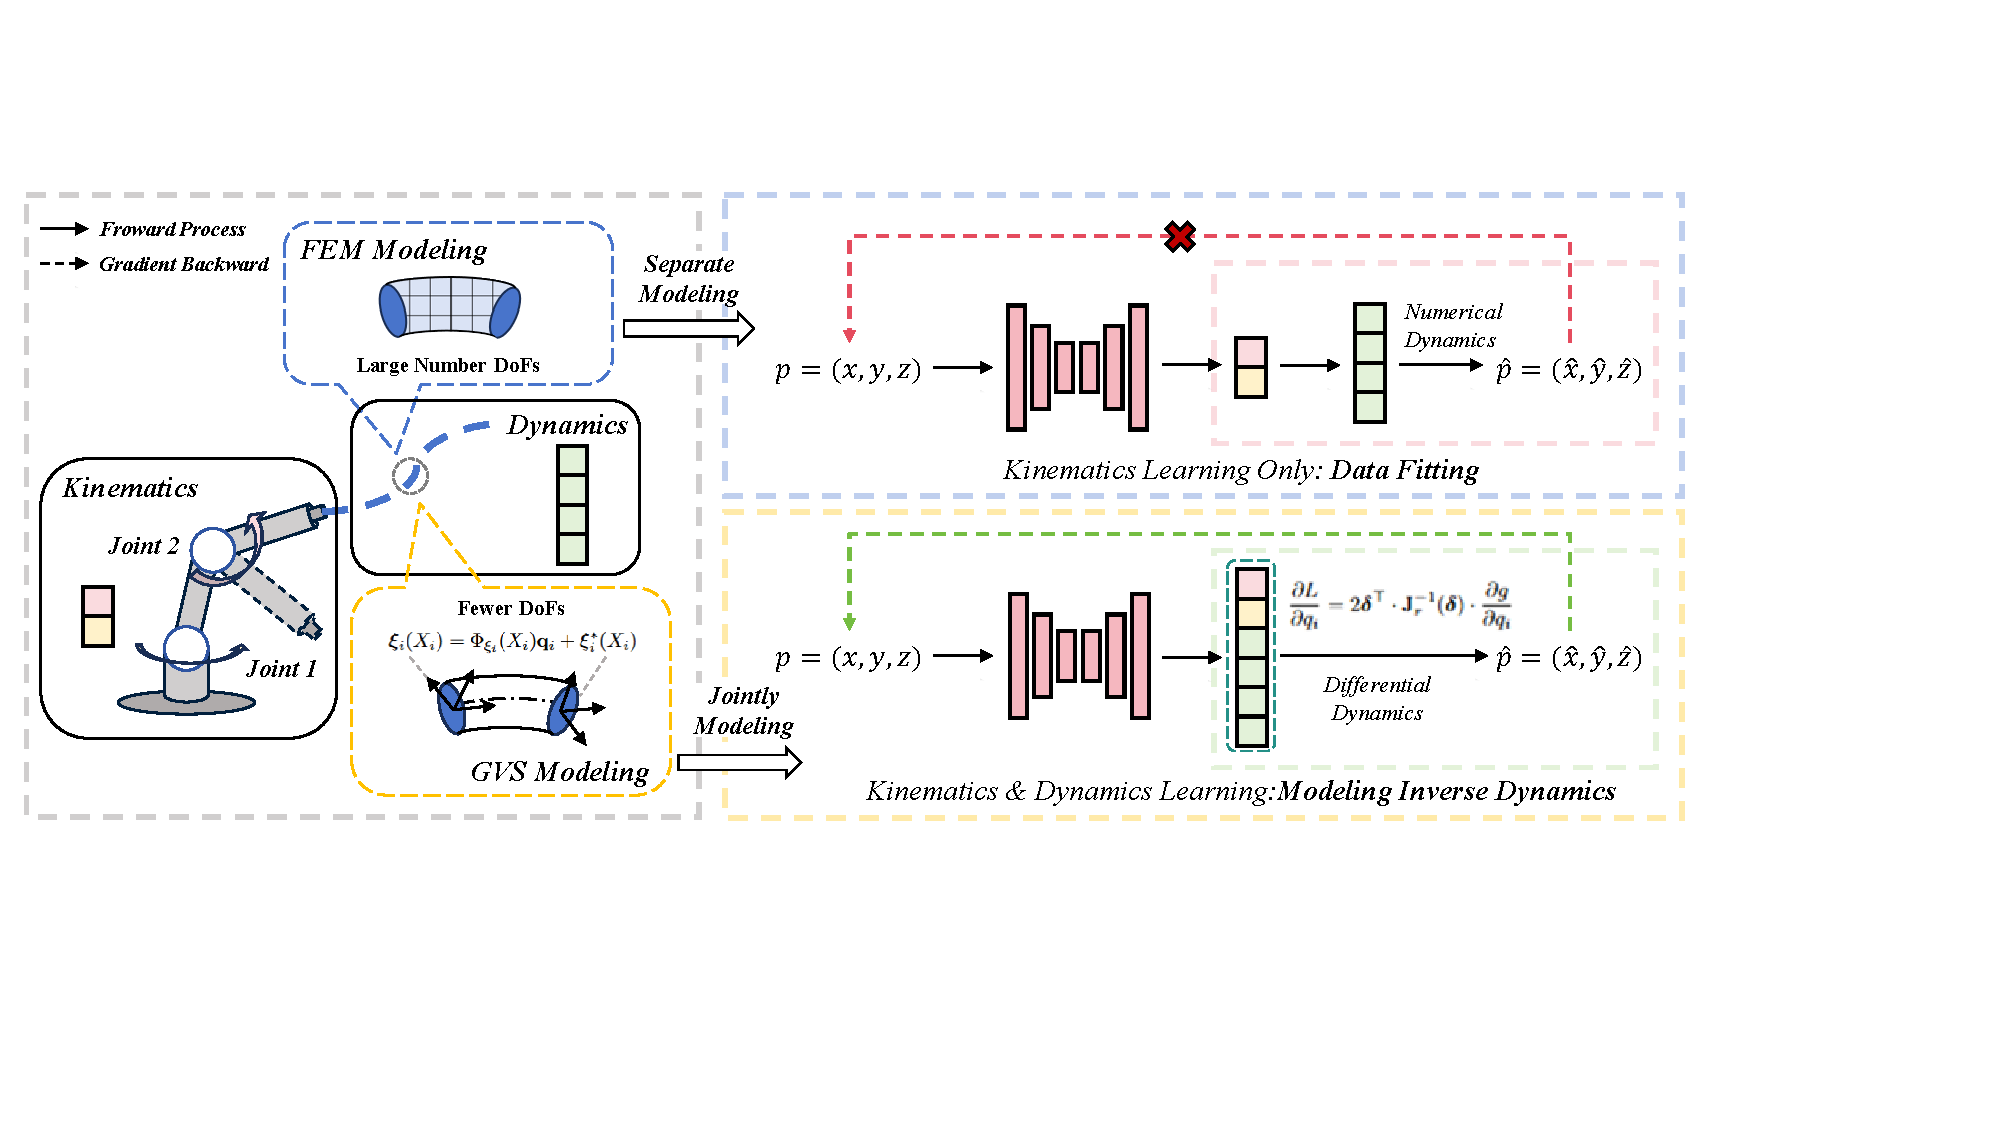
\includegraphics[width=0.95\linewidth]{./graph/top1.pdf} 
\vspace{-0.3cm}
\caption{We introduce the 3D dynamic manipulation benchmark for deformable objects by leveraging GVS modeling. This framework enables a reduced-DoF representation and differentiable system modeling, facilitating efficient learning of inverse dynamics. Our approach ensures consistency between kinematics and dynamics throughout the policy learning process.}
\vspace{-0.5cm}
\label{fig:top1}
\end{figure*}


\section{Related Work}
% 经典方法困境：揭示物理建模与优化的根本性计算瓶颈
% 数据驱动局限：指出学习范式因忽视物理先验导致的低效问题
% 新兴技术缺口：剖析扩散模型在动态物理约束建模中的不足
% → 最终锚定创新点：物理引导的降维扩散框架，同步突破三个维度的限制。

\subsection{Deformable Object Manipulation}
Early work in deformable object manipulation focused on quasi-static scenarios, often limited to 2D planes. These methods rely on vision-based inputs and hand-engineered dynamics tailored to specific tasks, such as cloth folding or rope knotting \cite{seita2020deep, hoque2022visuospatial, yin2021modeling}. While effective in constrained settings, they fall short in generalizing to high-speed or 3D environments.

Data-driven approaches have introduced learned representations of deformable states, often from visual observations or multimodal sensing (e.g., haptics, audio) \cite{grannen2021untangling, huang2023self, li2023see}. These enable tasks like cable reshaping and cloth folding \cite{jin2022robotic, xu2022dextairity}, but typically assume full observability or rely on expert demonstrations, limiting adaptability in dynamic or partially observed environments.

Unlike quasi-static tasks, dynamic manipulation leverages inertia and transient dynamics for high-speed motions such as whipping, throwing, or catching \cite{mason1986mechanics, jangir2020dynamic}. Optimization-based methods (e.g., iLQR, CHOMP) offer precision but are sensitive to modeling errors and lack robustness in real-world settings \cite{li2015folding, toussaint2018differentiable}. Iterative Learning Control (ILC) methods, like IRP \cite{chi2024iterative}, improve generalization via residual feedback but assume task repeatability and known Jacobians.


\subsection{Diffusion-Based Robotic Manipulation}
Diffusion models \cite{ho2020denoising} have emerged as a powerful framework in generative modeling, capable of accurately capturing complex, high-dimensional data distributions. They have achieved notable success in diverse domains such as image generation \cite{rombach2022high,peebles2023scalable}, video generation \cite{wang2025lavie,ma2024latte}, 3D shape synthesis \cite{pooledreamfusion}, and robotic policy learning \cite{chi2023diffusion,ze20243d}. 

In the context of robotic planning, particularly within complex and high-dimensional environments, diffusion-based generative models have been adopted to produce goal-conditioned action trajectories that better capture the stochasticity and flexibility needed for dynamic control \cite{chi2023diffusion, luo2024text}. Hierarchical approaches, such as the Hierarchical Diffusion Policy (HDP), further enhance this capability by coupling high-level task decomposition with kinematically-aware, low-level diffusion control, achieving competitive performance across a variety of manipulation tasks \cite{Ma_2024_CVPR}.

However, existing applications of diffusion policies have predominantly focused on quasi-static or fully actuated systems, thereby avoiding the complexities associated with underactuated and dynamically unstable manipulation scenarios.



% One of the foundational approaches in soft object manipulation relies on model-based methods, where the deformable object’s physical properties, such as elasticity, stiffness, and shape, are modeled explicitly. Early work focused on developing finite element models (FEM) to simulate soft materials and predict their behavior during manipulation tasks. These models have been successful in certain applications, but they often require significant computational resources and may struggle with real-time control in dynamic environments \cite{kim2017soft, ruggiero2018nonprehensile}.

% . Deep RL has been used to handle deformable objects by learning policies that maximize task-specific rewards, such as object stability or manipulation success \cite{andrychowicz2017hindsight, levine2016end}. However, RL methods often require large amounts of training data and may not generalize well across different object shapes or environmental conditions.




% The manipulation of deformable objects, particularly garments, remains a fundamental challenge in robotics due to high-dimensional state spaces and complex dynamics. Current approaches fall into two main categories: model-free and model-based methods. Model-free approaches, including reinforcement learning \cite{matas2018sim,jangir2020dynamic} and imitation learning \cite{avigal2022speedfolding,fu2024mobile,chi2023diffusion,ze20243d,pertsch2025fast}, learn direct observation-to-action mappings through end-to-end training. However, these methods struggle with precise shape control due to the lack of explicit object dynamics modeling. Model-based approaches require accurate state estimation \cite{shi2024robocraft,chen2021ab,shi2023robocook,shi2023robocook,huang2024spatio}, challenging when deformable objects like cloth exhibit severe self-occlusions. Furthermore, learning dynamics models demands extensive training data covering large state and action spaces. To overcome these challenges, we propose leveraging the expressive generative models, specifically diffusion models, for both full-state estimation from partial observations and dynamics modeling using large-scale simulation data.

%\subsection{Learning-Based Dynamics Models}

% Learning-based dynamics models aim to predict state transitions directly from interaction data, with the choice of state representation playing a critical role. Pixel-based representations frame the problem as action-conditioned video prediction \cite{yan2021learning}. However, these models often require extensive training data, are sensitive to occlusions, and struggle to generate physically plausible predictions due to the lack of explicit 3D structure \cite{yang2023learning}. In contrast, particle-based representations, like point clouds and meshes, offer a more structured and physically grounded approach to modeling deformable objects. These representations are typically processed using graph neural networks (GNNs), which model state transitions through message passing \cite{zhang2024adaptigraph,huang2022mesh,shi2024robocraft,shi2023robocook,ai2024robopack}. While GNNs have demonstrated effectiveness, we find that diffusion models provide a more scalable and expressive alternative, enabling accurate state transition learning from large-scale datasets and advancing deformable object dynamics modeling.


  


\section{Methods}
\textbf{Task Formulation.}
In this paper, we investigate rope whipping using one-dimensional deformable objects as a representative example. The task requires hitting a specified goal location in the air with the tip of a rope that is attached to a two-joint robotic arm.
Let  $\bm{Q} = \{\boldsymbol{q}_1, \boldsymbol{q}_2, \dots, \boldsymbol{q}_N\}  \in \mathbb{R}^{N\times D}$  represent the $N$ squences of the action vector of the robotic system with $D$ DoFs, which in this context specifically refers to the robot's joint angles. Let $\mathcal{F}: \mathbb{R}^{N\times D} \to \mathbb{R}^3$ denote the forward dynamics mapping, which transforms a given action $\boldsymbol{q}$ into a Cartesian-space position $\mathbf{p} = (x, y, z)^\top \in \mathbb{R}^3$:
\begin{equation}
 \mathcal{H}(x, y, z) = \bm{Q}.
\end{equation}
The objective of goal-conditioned dynamic manipulation is to learn or approximate an inverse mapping $\mathcal{H}: \mathbb{R}^3 \to \ \mathbb{R}^{N\times D}$, such that:

\begin{equation}
\mathcal{H}(\mathbf{p}) = \bm{Q}, \quad \text{where } \mathcal{F}(\bm{Q}) \approx \mathbf{p}.
\end{equation}
Here, $\mathcal{F}$ denotes the forward dynamics mapping from the robot's action space $\bm{Q}$ to a position $\mathbf{p} \in \mathbb{R}^3$ in Cartesian space. The goal is to find the optimal action $\bm{Q}$that drives the end-effector or deformable object to reach a desired goal location $\mathbf{p}$ in 3D space.



\begin{figure*}[t]
\centering
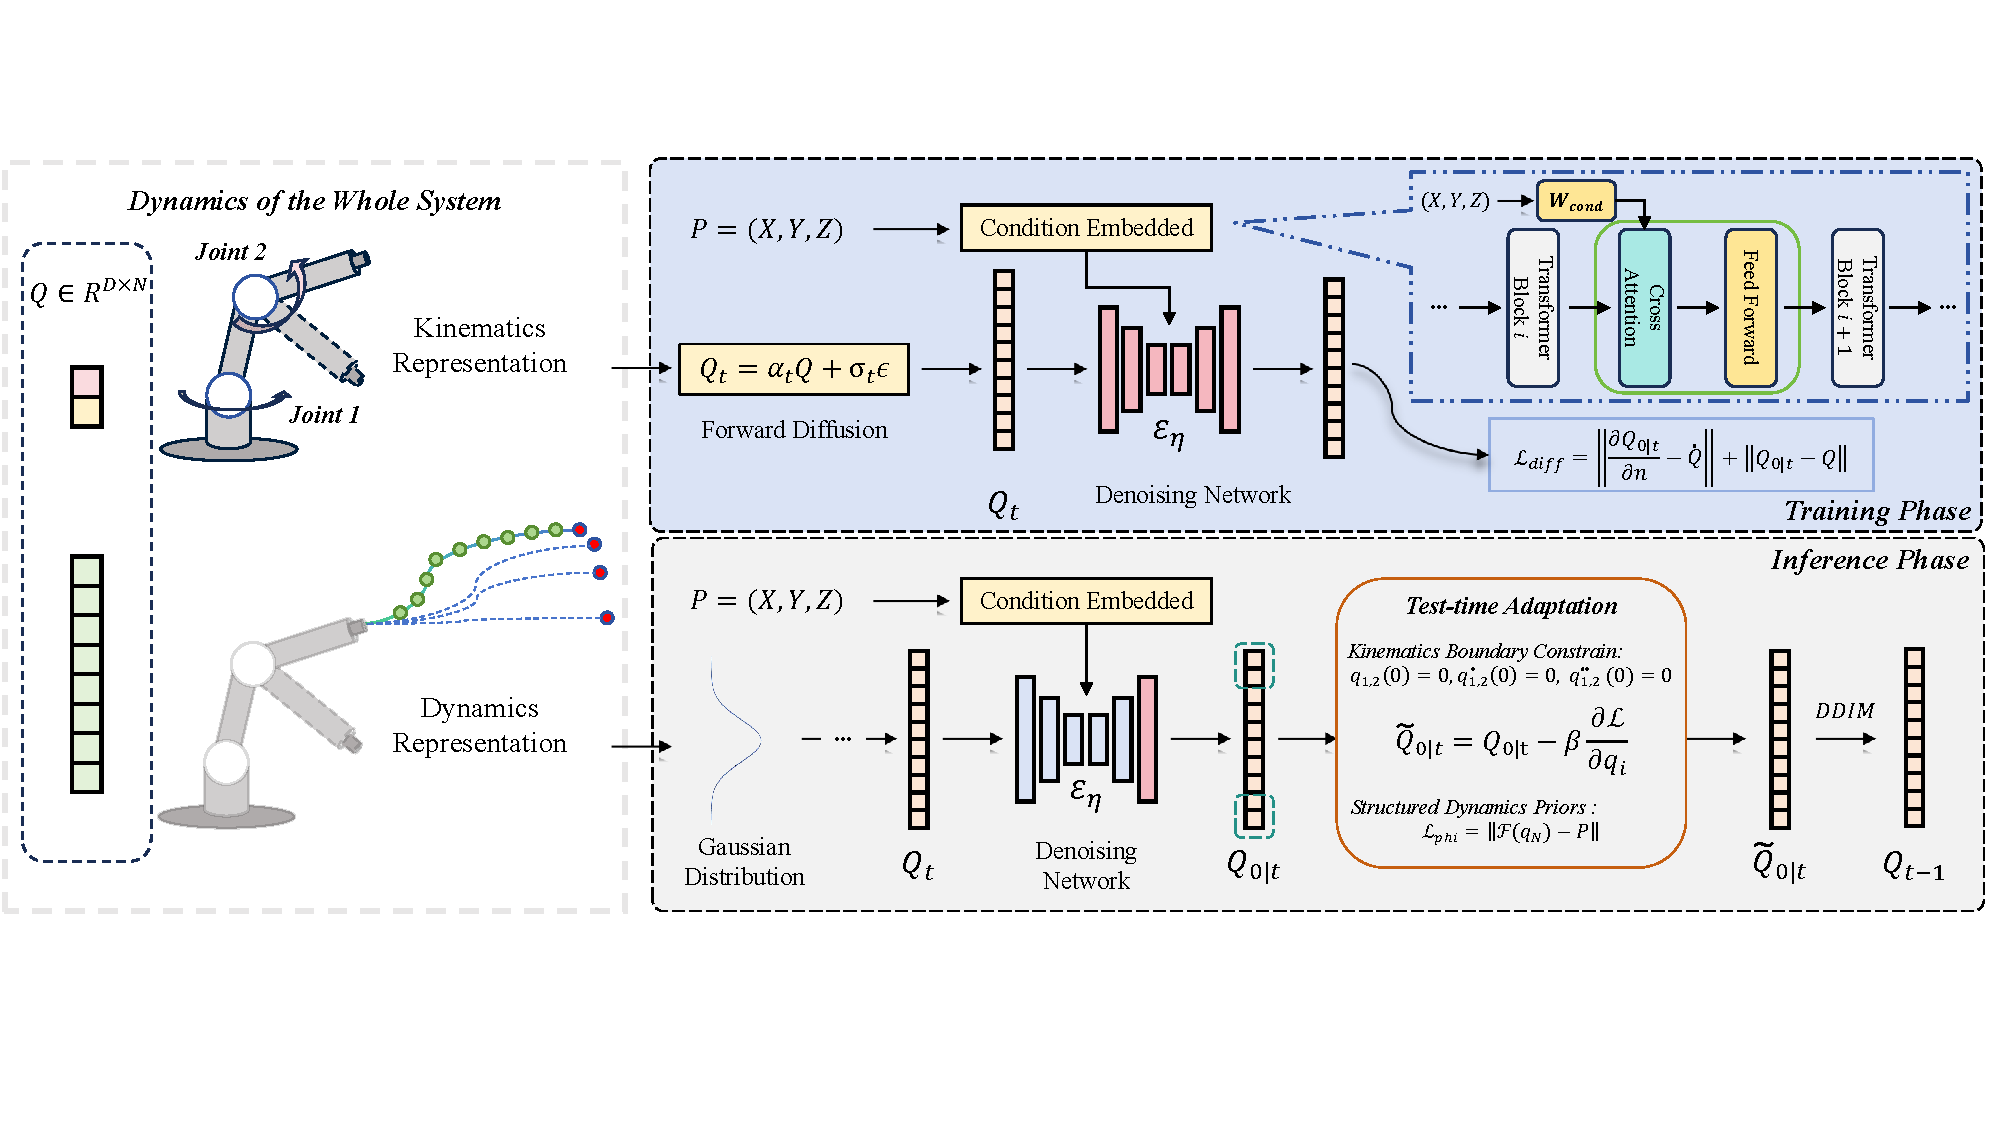
\includegraphics[width=0.95\linewidth]{./graph/nips_pipeline.pdf} 
\vspace{-0.2cm}
\caption{Pipeline of the Proposed DIDP Framework.
$D$ denotes the DoF of the entire system, and $N$ the length of the action sequence. In the denoising network $\epsilon_\eta$, the red blocks represent learnable parameters, while blue blocks indicate frozen modules. During the training phase, all parameters are optimized jointly. During the inference phase, we employ a test-time adaptation strategy by fine-tuning only the final projection layer.}
\vspace{-0.5cm}
\label{fig:main}
\end{figure*}


\subsection{Inverse Dynamics Modeling}

\textbf{Reduced-Order Modeling.}
Most prior works rely on traditional FEM to model deformable dynamics and generate simulation and training data. In FEM, the deformable body is discretized into a dense mesh of nodes, where the position field in $\mathbb{R}^3$ is interpolated over these nodes, resulting in a high-dimensional system with a large number of DoFs. This high dimensionality significantly increases the difficulty of learning effective policies. Furthermore, previous works often model the grid and deformable components separately, which hinders the integration of physics-informed learning strategies~\cite{irp}. In this work, following~\cite{Anup2025reduced}, we adopt the GVS model to construct the simulator and prepare training data, achieving a significant reduction in the system’s state dimensionality. Below, we briefly revisit the GVS formulation.

The GVS model directly parameterizes the distributed strain field in  Lie algebra $\boldsymbol{\xi}_i \in \mathfrak{se}(3)$ using a finite set of generalized coordinates $\boldsymbol{q}_i \in \mathbb{R}^{D}$ and a set of basis functions $\Phi_{\xi_i}$. Based on this formulation, the configuration $\mathbf{g} \in SE(3)$ in the grid part can be recursively computed:
\begin{equation}
\boldsymbol{\xi}_i = \Phi_{\xi_i} \boldsymbol{q}_i + \boldsymbol{\xi}_i^*, \quad \mathbf{g}_i = \mathbf{g}_{i-1} \exp(\hat{\boldsymbol{\xi}_i})
\label{eq: grid}
\end{equation}
Here, $\boldsymbol{\xi}_i^*$ denotes a reference strain field, which can incorporate constraints such as inextensibility. The operator $\hat{\boldsymbol{\xi}}_i$ maps from $\mathfrak{se}(3)$ to $SE(3)$. This formulation enables the soft link configuration using only essential deformation modes. For the deformable objects parts, the $\mathbf{g} \in SE(3)$ can be recursively computed as following:
\begin{equation}
\mathbf{g}_i = \mathbf{g}_{i-1}\exp(\widehat{\Omega}_i),
\label{eq: soft}
\end{equation}
where $\widehat{\Omega}_i$ is computed via a truncated Magnus expansion of the strain field. Compared to FEM, which requires a large number of nodal displacements to capture fine-scale deformation, the strain-based GVS model achieves comparable accuracy with significantly fewer DoFs. Using $\boldsymbol{q}$ and the differential kinematic equations, the generalized Lagrangian equation of the robots dynamics is derived \cite{Anup2025reduced}:
\begin{equation}
\mathbf{M}(\boldsymbol{q}) \ddot{\boldsymbol{q}} + \mathbf{C}(\boldsymbol{q}, \dot{\boldsymbol{q}}) \dot{\boldsymbol{q}} + \mathbf{K}(\boldsymbol{q}) = \mathbf{B}(\boldsymbol{q}) \mathbf{u} + \mathbf{F}_{\text{ext}},
\end{equation}


\textbf{On the Choice of the Learning Space. } In many prior works on deformable object manipulation, the two joints of the robotic arm are treated as controllable, while the deformable object itself is considered uncontrollable. As a result, these methods often take observations of the deformable object as input and predict actions for the robotic joints. However, this decoupled formulation limits the expressiveness of the learned inverse dynamics, as the input-output mapping is not sampled from the full system's inverse dynamics. In this paper, we propose to jointly model the robot and the deformable object as a unified system. By directly predicting the joint angles $\bm{q}$, which include both the robotic arm and deformable components, our approach captures the full inverse dynamics more effectively and leads to improved learning performance. Thus, we consider the 20-DoF $\bm{Q} = \{\boldsymbol{q}_1, \boldsymbol{q}_2, \dots, \boldsymbol{q}_N\}  \in \mathbb{R}^{N\times 20}$ to describe the whole dynamics. Each vector $\boldsymbol{q}_i$ represents a 20-DoF action at $i-th$ squence of the overall actions. Where the $N$ denote the length of the sequence of the actions and $D$ denote the DoF of the whole dynamics systems, in which the first 2 DoF is used for the grid parts and the following are used to discribe the deformable objects parts. 


\textbf{Diffusion-based Training.}
The diffusion model represents data through a stochastic process. Let $\bm{Q}_{0}$ denote a real robotic action, the forward diffusion process aims to generate a sequence of noisy latent variables $\bm{Q}_1,\bm{Q}_2, ..., \bm{Q}_T$ using a Markovian process, defined as:
\begin{equation}
    \begin{aligned}
        \bm{Q}_t = \alpha_t \bm{Q}_0 + \sigma_t\epsilon ,
    \end{aligned}	
    \label{eq: c-ddpm-forward}
\end{equation}
where $ \alpha_t \in(0,1)$ represents the noise schedule, $\sigma_t$ denotes the covariance at $t$, and $\epsilon$ represents the Gaussian noise. During training, the diffusion loss aims to maximize the likelihood of the sample results by using the variational lower bound. In the reverse process, we incorporate the position of the goal condition $ \bm{p}$ as the conditioning of the score functions $\epsilon_\eta(\bm{Q}_t, \bm{p}, t)$ and predict the robotic actions iteratively:

In the vanilla diffusion model\cite{dhariwal2021diffusion}, the denoising network is trained to predict the Gaussian noise and the recover the clean data using:
\begin{equation}
    \begin{aligned}
      \bm{Q}^\eta_{0|t}= \frac{\bm{Q}_t - \sigma_t\epsilon_\eta(\bm{Q}_t, \bm{p}, t)}{\alpha_t} .
    \end{aligned}	
    \label{eq: c-ddpm-reserved}
\end{equation}
Our diffusion policy is designed to directly predict the clean action sequence $\bm{Q}^\eta_{0|t}$. In addition, the angular velocity term $\bm{Q}_d$ is incorporated to enable second-order training, allowing the model to better capture dynamic behaviors:
\begin{equation}
    \begin{aligned}
    \mathcal{L}_{\text{diff}}&= \lambda_{Q}\|\bm{Q} -\bm{Q}^\eta_{0|t}\|_2^2 + \lambda_{Q_d}\|\bm{Q}_d -\dot{\bm{Q}}^\eta_{0|t}\|_2^2 ,\\
    \end{aligned}
\end{equation}


\begin{comment}
    \subsection{Network Designing}
We adopt a Transformer-based architecture as the denoiser of the diffusion policy, incorporating both cross attention and causal attention to effectively model the temporal structure and goal-conditioning in action prediction tasks.

\textbf{Cross Attention for Conditioning. } To ensure the model generates goal-directed actions, we employ \textit{cross attention} layers that inject goal information into each denoising step. 

\textbf{Autoregressive Action Prediction. } 
From a sequential modeling perspective, the generation process naturally follows an \textit{autoregressive factorization} of the conditional distribution:
\begin{equation}
    p(\bm{Q}_t \mid \bm{P}) = \prod_{i=1}^{T} p(\boldsymbol{q}_i \mid \boldsymbol{q}_{<i}, \bm{P})
\end{equation}

To capture this structure within our Transformer-based denoiser, we employ \textbf{causal self-attention}, which ensures that each token $\boldsymbol{q}_i$ attends only to itself and preceding tokens $\{\boldsymbol{q}_1, \dots, \boldsymbol{q}_{i-1}\}$. This structure is particularly suitable for modeling sequences of actions, where temporal causality must be strictly preserved for realistic and physically valid generation.

\end{comment}


 
\subsection{Differential Dynamics Prior from GVS model.} 
For goal-conditioned dynamic manipulation of deformable objects, it is essential to impose constraints in Cartesian space to ensure that the robot's joint movements correspond to the desired deformation behavior. Achieving this requires the system dynamics to be differentiable, enabling effective gradient-based policy optimization.

Revisiting the GVS model introduced in \cref{eq: grid} and \cref{eq: soft}, the position of any point on the end-effector can be directly obtained via $\bm{p} = \mathbf{g}_N(1\!:\!3,4)$. The dynamics prior aims to enforce consistency between the predicted pose $g^\eta_N$ and the goal pose $\tilde{g}_N$. To this end, we define the following loss function:
\begin{equation}
\mathcal{L}_{\text{pos}}= \left\| \log\left( \tilde{g}_N^{-1} \cdot g^\eta_N \right) \right\|^2,
\end{equation}
which penalizes discrepancies between the predicted and goal transformations in the Lie algebra. This loss is differentiable proved by the following corollary.


\begin{corollary} 
\label{cor:differentiable}
$\mathcal{L}_\text{pos}$ is differentiable with respect to the joint variables $\mathbf{q}_i$, i = 1, ..N.
\end{corollary}
\textbf{Proof.} 
Let:\[\boldsymbol{\delta} = \log\left( \tilde{\mathbf{g}}_N^{-1} \cdot \mathbf{g}^\eta_N \right)\]
Using the chain rule and the differential of the Lie logarithm, the gradient of the loss function with respect to joint variables $q_i$ can be approximated as:
\begin{equation}
\frac{\partial \mathcal{L}_{\text{pos}}}{\partial q_i} = 2 \boldsymbol{\delta}^\top \cdot \frac{\partial \boldsymbol{\delta}}{\partial q_i}  \approx 2 \boldsymbol{\delta}^\top \cdot \mathbf{J}_r^{-1}(\boldsymbol{\delta}) \cdot \frac{\partial \mathbf{g}_N}{\partial q_i}, \quad i = 1, ..N
\end{equation}
where $\mathbf{J}_r^{-1}(\cdot)$ denotes the inverse of the right Jacobian of the Lie group $\mathrm{SE}(3)$. Thus, the differentiability of $\frac{\partial \mathbf{g}_N}{\partial q_i}$ is sufficient for enabling gradient-based policy optimization. Recall from \cref{eq: grid} and \cref{eq: soft} that the dynamics of the grid and soft segments are modeled as:
\begin{equation}
\mathbf{g}_N = \exp(\hat{\boldsymbol{\xi}}_1) \cdot \exp(\hat{\boldsymbol{\xi}}_2) \cdot \exp(\widehat{\Omega}_3) \cdots \exp(\widehat{\Omega}_N).
\end{equation}
$\widehat{\Omega}_i$ can be computed via a truncated Magnus expansion. A fourth-order approximation is given by:
\begin{equation}
\widehat{\Omega}_i= \frac{H}{2}(\xi^1_i + \xi^2_i) + \frac{\sqrt{3} H^2}{12} [\xi^1_i, \xi^2_i],
\end{equation}
with $H$ being the discretization step size and $[\cdot,\cdot]$ denoting the Lie bracket capturing non-commutative effects. Here, $\xi^1_i$ and $\xi^2_i$ are  Zannah collocation points along the soft body. 
For the grid components with $i = 1, 2$, The partial derivative of the end-effector pose $\mathbf{g}_N$ with respect to the generalized coordinate $\boldsymbol{q}_1$ is given by:
\begin{equation}
\begin{aligned}
\frac{\partial \mathbf{g}_N}{\partial \boldsymbol{q}_1}
&= \left( \frac{\partial \exp(\hat{\boldsymbol{\xi}}_1)}{\partial \boldsymbol{q}_1} \right)
\cdot \exp(\hat{\boldsymbol{\xi}}_2)
\cdot \prod_{i=3}^{N} \exp(\widehat{\Omega}_i) \\
&= 
\exp(\hat{\boldsymbol{\xi}}_1), \cdot \mathbf{J}_l(\boldsymbol{\xi}_1) \cdot \Phi_{\xi_1} \cdot \exp(\hat{\boldsymbol{\xi}}_2) \cdot \prod_{i=3}^{N} \exp(\widehat{\Omega}_i)
\end{aligned}
\end{equation}
where $ \mathbf{J}_l(\boldsymbol{\xi}_1)$ is the left Jacobian associated $\boldsymbol{\xi}_1$.
For the deformable segments, indexed by $i = 3, 4, \ldots, N$, the partial derivative of the end-effector pose $\mathbf{g}_N$ with respect to the local generalized coordinate $\boldsymbol{q}_i$ is given by:
\begin{equation}
\frac{\partial \mathbf{g}_N}{\partial \boldsymbol{q}_i}
=
\left( \prod_{k=1}^{2} \exp(\widehat{\xi}_k) \right)\left( \prod_{k=3}^{i-1} \exp(\widehat{\Omega}_k) \right)
\cdot \mathbf{J}_{\text{l}}(\Omega_i)
\cdot \frac{\partial \Omega_i}{\partial \boldsymbol{q}_i}
\cdot \exp(\widehat{\Omega}_i)
\cdot \left( \prod_{k=i+1}^{N} \exp(\widehat{\Omega}_k) \right).
\end{equation}
$\mathbf{J}_{\text{l}}(\Omega_i)$ denotes the left Jacobian associated with $\Omega_i$. Assuming that the basis components $\boldsymbol{\xi}_i^1$ and $\boldsymbol{\xi}_i^2$ are differentiable with respect to $\boldsymbol{q}_i$, the partial derivative $\frac{\partial \Omega_i}{\partial \boldsymbol{q}_i}$ is well-defined and exists.








\subsection{The Physical Informed Test-Time Adaptation.}
In many real-world domains, especially in robotics and physical trajectory generation, diffusion models pre-trained via imitation learning can produce behaviorally plausible samples but may fail to satisfy strict physical or structural constraints at inference time. To mitigate this issue without disrupting the learned dynamics, we propose a \textit{physically informed test-time adaptation} (PITA) strategy that introduces lightweight structural regularization during the sampling process.

\textbf{Kinematic Boundary Condition.}
The zero-angle configuration typically corresponds to a standardized initial pose in many robotic platforms. Enforcing this condition ensures consistent and interpretable starting configurations across trajectories.
We need to enforce that $\bm{Q}(0)=0, \dot{\bm{Q}}(0)=0, \ddot{\bm{Q}}(0)=0$, which can be modeled as L2 regularization as a term of loss function $\mathcal{L}_{KBC}$.

\textbf{Test-Time Adaptation for Diffusion Sampling Process.}
Given a pre-trained diffusion model that predicts a denoised trajectory $\bm{Q}_{0|t}$ from a noisy sample $\bm{Q}_t$, we consider the incorporation of physical observations represented by $\bm{p}$. These observations depend on the clean trajectory through a known differentiable dynamics model $\bm{p} = \mathcal{F}(\bm{Q}_{0|t})$.

We aim to sample from the posterior distribution $p(\bm{Q}_t \mid \bm{p})$, which integrates the generative prior $p(\bm{Q}_t)$ with a physically grounded likelihood $p(\bm{p} \mid \bm{Q}_{0|t})$. For example, the likelihood can be instantiated as a soft constraint based on a differentiable loss function $\mathcal{L}(q_1, q_2)$, where $q_1, q_2$ are specific joint configurations extracted from $\bm{Q}_{0|t}$. This gives:
\[
p(\bm{p} \mid \bm{Q}_{0|t}) \propto \exp\left(-\mathcal{L}(q_1, q_2)\right).
\]

To guide the sampling process under this posterior, we apply the identity from score-based generative modeling to approximate the posterior score:
\begin{equation}
\begin{aligned}
    \nabla_{\bm{Q}_t} \log p(\bm{Q}_t \mid \bm{p}) &\approx \nabla_{\bm{Q}_t} \log p(\bm{Q}_t) + \nabla_{\bm{Q}_{t}} \log p(\bm{p} \mid \bm{Q}_{t})\\
   & =\nabla_{\bm{Q}_t} \log p(\bm{Q}_t) +  \frac{\partial \mathcal{L}(q_1, q_2)}{\bm{Q}_{0|t}} \cdot \frac{\partial \bm{Q}_{0|t}}{\partial \bm{Q}_t},
\end{aligned}
\label{eq:posterior_score}
\end{equation}
Since $\bm{Q}_{0|t}$ is the output of the diffusion policy, and the differentiability of $\frac{\partial \mathcal{L}(q_1, q_2)}{\partial \bm{Q}_{0|t}}$ has been established in  Corollary~\ref{cor:differentiable}, the full gradient $\frac{\partial \mathcal{L}(q_1, q_2)}{\partial \bm{Q}_t}$ can be computed via the chain rule by propagating through the denoiser network. To ensure stable test-time adaptation, we restrict gradient updates to only the final projection layer of the denoiser network. The final loss function for test-time adaptation $\mathcal{L}(q_1, q_2)$ is as following:
\begin{equation}
\mathcal{L}= \mathcal{L}_{\text{pos}} + \mathcal{L}_{\text{KBC}},
\end{equation}

Equation~\ref{eq:posterior_score} enables physically informed guidance at each sampling step by modifying either the sample $\bm{Q}_t$ or the model parameters, thereby enforcing consistency with domain-specific physical constraints during test-time inference.
 







% The dataset features three distinct material classes representing fundamental variations in compliance and damping characteristics: Class A (Hemp) with high stiffness ($E=1.0$MPa) and moderate damping, Class B (Nylon) with intermediate stiffness ($E=0.5$MPa) and balanced damping, and Class C (Rubber) with low stiffness ($E=0.1$MPa) and high damping. Each class contains exactly 55,000 trajectories, implemented through distinct constitutive parameters in our viscoelastic rod model (see Table~\ref{tab:material_properties}). All data is stored in compressed HDF5 format containing: the control input matrix $\theta$, full state trajectory $\texttt{qqd} \in \mathbb{R}^{L\times2n}$, Cartesian positions/velocities $\texttt{pos/vel} \in \mathbb{R}^{L\times21\times3}$, material class label, and timestep information. This comprehensive dataset supports diverse research applications including learning dynamic models, control policy optimization, system identification, and long-horizon prediction tasks in soft continuum robotics.



%\begin{table}[t]
%\centering
%\caption{Material Properties of Three Rope Classes}
%\begin{tabular}{lccc}
%\hline
%\textbf{Property} & \textbf{Class A (Hemp)} & \textbf{Class B (Nylon)} & \textbf{Class C (Rubber)} \\
%\hline
%Length $L$ (m) & 0.5 & 0.5 & 0.5 \\
%Radius $r(x)$ (m) & $0.015 - 0.010x$ & $0.01 - 0.007x$ & $0.012 - 0.005x$ \\
%Young's Modulus $E$ (Pa.s) & $1.0 \times 10^6$ & $5.0 \times 10^5$ & $1.0 \times 10^5$ \\
%Shear Modulus $G$ (Pa) & $3.33 \times 10^5$ & $1.67 \times 10^5$ & $3.33 \times 10^4$ \\
%Poisson Ratio & $0.5$ & $0.45$ & $0.4$ \\
%Viscous Damping $\eta$ & $1.0 \times 10^4$ & $2.0 \times 10^4$ & $4.0 \times 10^4$ \\
%Density $\rho$ (kg/m$^3$) & $1000$ & $800$ & $1200$ \\
%\hline
%\end{tabular}
%\label{tab:material_properties}
%\end{table}

\begin{comment}
    \begin{table}[t]
\centering
\caption{Material Properties of Five Rope Classes}
\resizebox{0.9\textwidth}{!}{\begin{tabular}{lccccc}
\hline
\textbf{Property} & \textbf{Hemp} & \textbf{Nylon} & \textbf{Rubber} & \textbf{Silicone} & \textbf{Kevlar} \\
\hline
Length $L$ (m) & 0.5 & 0.5 & 0.5 & 0.5 & 0.5 \\
Radius $r(x)$ (m) & $0.015 - 0.010x$ & $0.01 - 0.007x$ & $0.012 - 0.005x$ & $0.011 - 0.004x$ & $0.013 - 0.009x$ \\
Young's Modulus $E$ (Pa) & $1.0 \times 10^6$ & $5.0 \times 10^5$ & $1.0 \times 10^5$ & $5.0 \times 10^4$ & $5.0 \times 10^7$ \\
Shear Modulus $G$ (Pa) & $3.33 \times 10^5$ & $1.67 \times 10^5$ & $3.33 \times 10^4$ & $1.67 \times 10^4$ & $1.67 \times 10^7$ \\
Poisson Ratio & $0.5$ & $0.45$ & $0.4$ & $0.49$ & $0.35$ \\
Viscous Damping $\eta$ & $1.0 \times 10^4$ & $2.0 \times 10^4$ & $4.0 \times 10^4$ & $5.0 \times 10^4$ & $1.0 \times 10^4$ \\
Density $\rho$ (kg/m$^3$) & $1000$ & $800$ & $1200$ & $1100$ & $1440$ \\
\hline
\end{tabular}}
\label{tab:material_properties}
\end{table}


\end{comment}


\section{Experiments}
\subsection{Dataset}

\begin{figure*}[t]
\centering
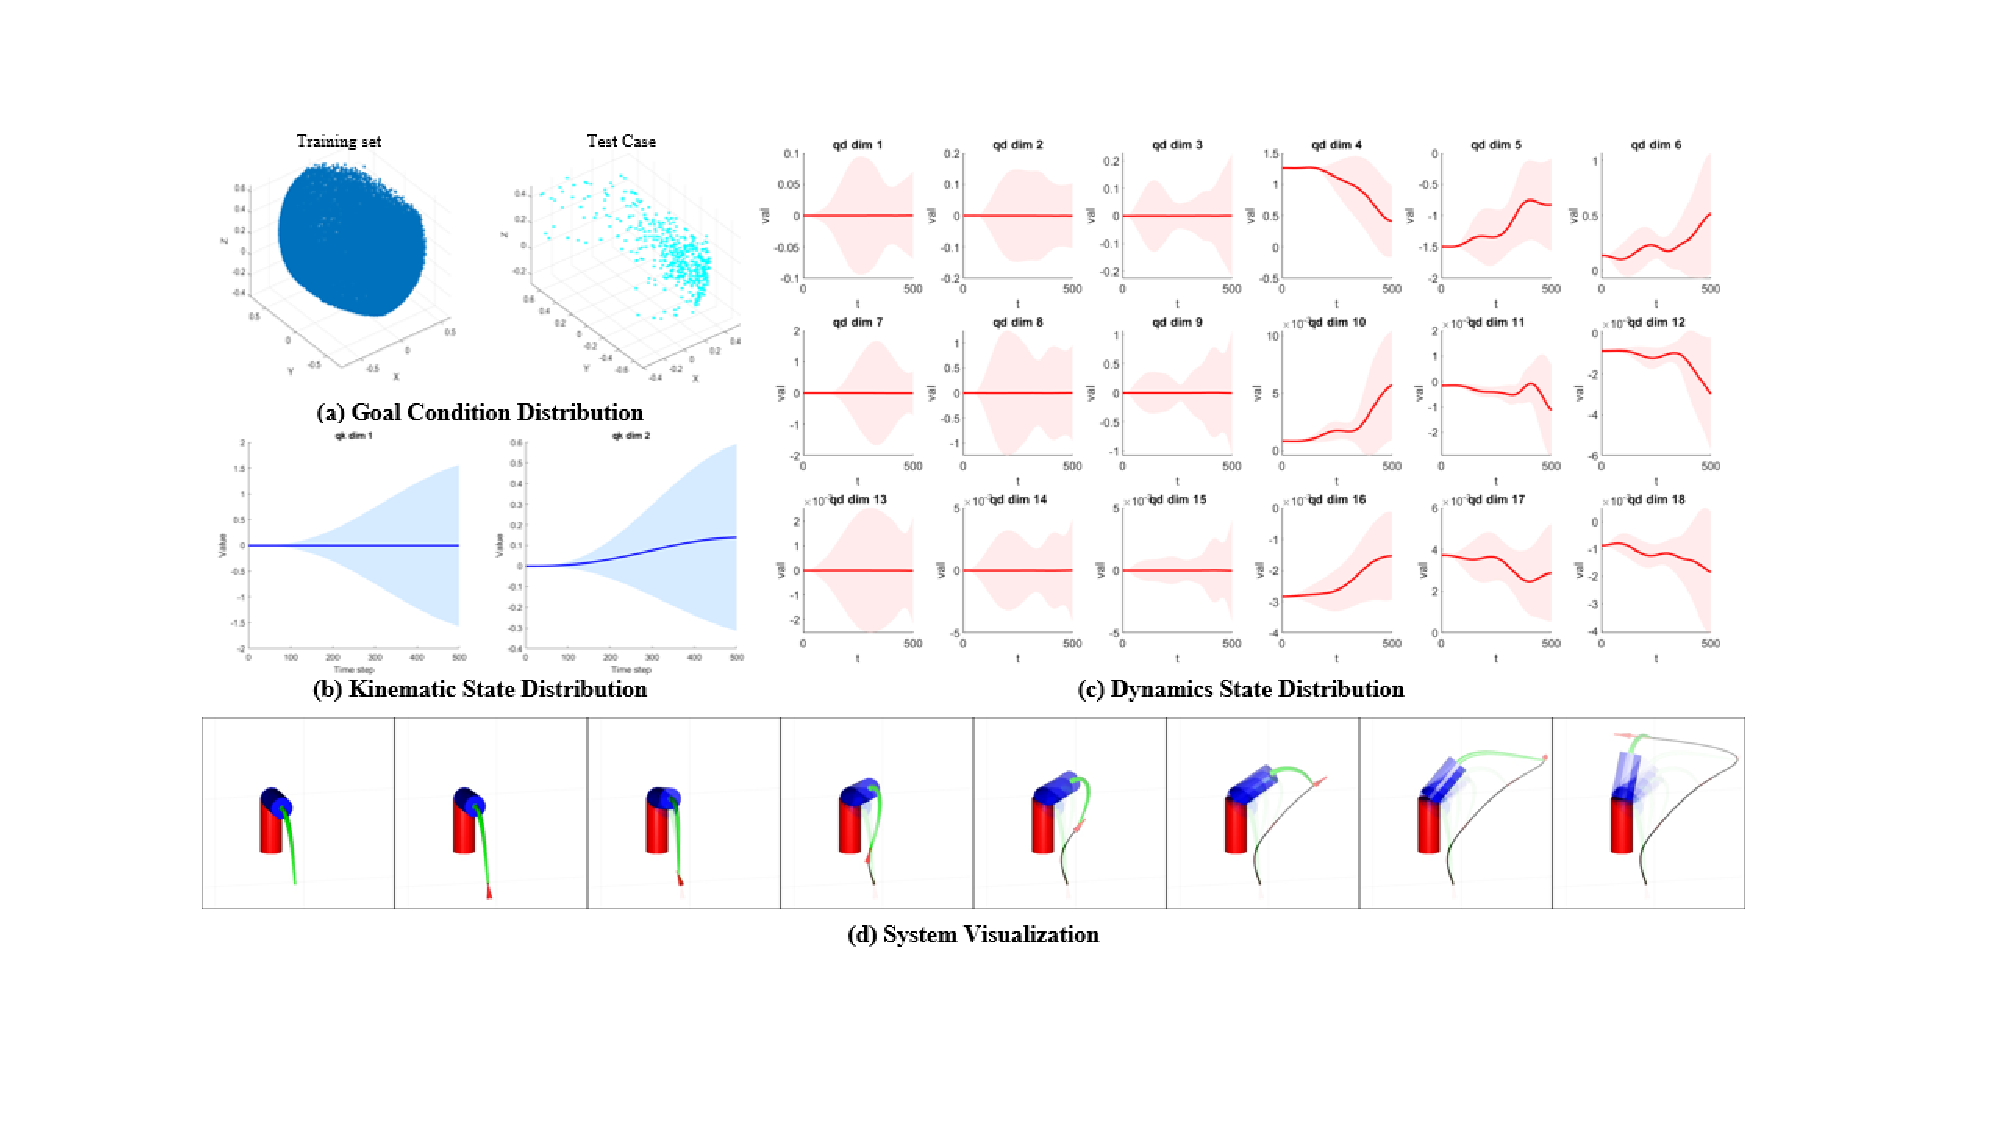
\includegraphics[width=0.95\linewidth]{./graph/dataset.pdf} 
\vspace{-0.3cm}
\caption{Dataset overview. (a) shows the distribution of goal conditions in 3D space for both training and testing cases, demonstrating comprehensive spatial coverage. (b) and (c) depict the distributions of kinematic and dynamic states, respectively. The curves indicate the mean and standard deviation across time steps, based on a reduced representation with 20 DoFs to describe the entire system. (d) provides a visualization of the complete system within the simulation environment.}
\vspace{-0.5cm}
\label{fig:dataset}
\end{figure*}
\textbf{Overview.} 
Our benchmark dataset comprises $N=55{,}000$ high-fidelity simulated trajectories of a whip-like continuum soft robot, as shown in Figure~\ref{fig:dataset}. Each trajectory is generated by first sampling an actuation input matrix $\theta \in \mathbb{R}^{2\times4}$ uniformly from the operational input space, then simulating the system's dynamic response over $t\in[0,T]$ using a Cosserat rod-based physics engine. Simulations run for $T=0.5$s using a fixed timestep $\Delta t = 0.001$s (RK4), resulting in $L=500$ time steps. At each time step, we record the complete configuration state $\boldsymbol{Q}\in \mathbb{R}^{N\times D}$, velocity state $\dot{\boldsymbol{Q}}\in \mathbb{R}^{N\times D}$, and the Cartesian positions and velocities of 21 evenly spaced material points. % This yields time-series data tensors of shape $L\times21\times3$ for both positions and velocities.


\textbf{Sampling Strategy.} 
To comprehensively capture the spatial and temporal diversity of soft continuum robot dynamics, we propose a structured yet randomized sampling strategy that generates large-scale sequences. Each control input is represented as a parameter matrix $\boldsymbol{q} \in \mathbb{R}^{2 \times 4}$, where the two rows correspond to the independently actuated joints of the robot, and the four columns encode piecewise-constant actuation commands over four equal-duration temporal segments.

Control inputs are structured as $\boldsymbol{q} \in \mathbb{R}^{2 \times 4}$, with each row encoding actuation for one joint over four temporal segments. Candidate matrices are drawn from joint-specific uniform distributions: $\boldsymbol{q}_1 \sim \mathcal{U}[-\pi, \pi]$ and $\boldsymbol{q}_2 \sim \mathcal{U}[-\pi/2, \pi/4]$. To ensure stability and physical validity, trajectories with numerical errors or divergence are filtered. Valid samples are simulated using a stiff-aware solver (\texttt{ODE15s}) with Jacobian-based evaluations.

% To construct the sampling space, we draw 100{,}000 candidate $\boldsymbol{q}$ matrices from joint-specific uniform distributions that reflect realistic joint limits: the first joint is sampled from $\boldsymbol{q}_1 \sim \mathcal{U}[-\pi, \pi]$, and the second from  $\boldsymbol{q}_2 \sim \mathcal{U}[-\pi/2, \pi/4]$. These choices encode both symmetry and asymmetry in actuation range, promoting spatial diversity in the resulting robot motions across the dataset. To enforce physical plausibility and ensure bounded motion profiles, each generated trajectory undergoes rigorous filtering  at any point in time.Moreover, any candidate leading to numerical instability, NaNs, or solver divergence in simulation is excluded. Validated control inputs are then passed into a high-fidelity dynamic simulator leveraging stiff-aware integration with \texttt{ODE15s}, which includes Jacobian-based evaluations for accurate modeling of nonlinear robot dynamics.


% Figure~\ref{fig:dataset} summarizes the dataset. (a) demonstrates spatial diversity across goal states. (b)–(c) show low-dimensional kinematic and dynamic trends over time. (d) visualizes typical deformations, reflecting the system’s complexity and variability under diverse actuation inputs.



% Each simulation generates a rich spatial structure of the robot’s state evolution. At each time step, the full body kinematics are resolved via the robot-specific Jacobian and twist-based forward kinematics, yielding spatially-resolved position and velocity fields across the soft backbone. These data are stored alongside the governing parameters ($\boldsymbol{q}$, $T$) and system state ($q$, $\dot{q}$) for use in downstream learning and evaluation. All trajectories are saved in a structured format (HDF5) with consistent chunking for efficient retrieval and processing.

 
 
\textbf{Evaluation Metrics.} We use the Euclidean distance between the rope's tip and the goal position in Cartesian space as the primary evaluation metric. To assess performance under varying precision requirements, we define success based on distance thresholds of 10\,cm, 5\,cm, 2\,cm, and 1\,cm. The success rate is computed as the percentage of trials in which the rope tip falls within each specified threshold. This multi-level evaluation provides a comprehensive assessment of both coarse and fine-grained control capabilities.



\subsection{Validation on the Learning Space.}
\textbf{Experimental Settings.} We evaluate the effectiveness of different learning spaces using a diffusion policy with a Transformer-based denoiser. We compare two settings:

\textit{Kinematics}: The policy is trained solely on the kinematic states, i.e., it learns to replicate the behavior of the robot’s actuated joints without considering the deformable rope.

\textit{Kinematics + Dynamics}: The policy is trained on both the robot and the rope using the reduced-order dynamics model, thereby capturing the full system behavior.

\textbf{Experimental Analyisis.} Note that the kinematics-only model lacks dynamic state representations, and therefore cannot leverage our test-time adaptation strategy. Despite this, as shown in \cref{tab: Learning_Space}, extending the learning space to include dynamics yields substantial performance improvements. This highlights the value of incorporating physically meaningful inverse dynamics: it not only enhances interpretability but also significantly boosts imitation learning performance.
\begin{table}[t]
\centering
\vspace{-0.4cm}
\resizebox{0.9\textwidth}{!}{\begin{tabular}{cc|cc|c|cccc}
\toprule
\multirow{2}{*}{Kinematic} & \multirow{2}{*}{Dynamics}        & \multirow{2}{*}{DDIM}       & \multirow{2}{*}{TTA}       & \multirow{2}{*}{Distance} & \multicolumn{4}{c}{Success Rate}   \\ \cline{6-9}
&         &         &  &            & 10 cm  & 5cm    & 2 cm   & 1 cm  \\ \midrule
\checkmark    &                           & \checkmark   &  & 0.065                        & 0.773  & 0.699  & 0.434  & 0.107          \\ 
\checkmark & \checkmark & \checkmark &                           & 0.041                        & 0.884  & 0.800  & 0.616  & 0.190 \\
\checkmark & \checkmark &                           & \checkmark & 0.036                     & 0.939  & 0.843  & 0.623  & 0.208 \\ \midrule
\end{tabular}}
\caption{Quantitative comparison of learning spaces. The extending the learning space to include dynamics leads to significant improvements in task performance.}
\vspace{-0.8cm}
\label{tab: Learning_Space}
\end{table}

\subsection{Validation on the Learning Strategy.}
\textbf{Experimental Settings.} We evaluate the effectiveness of different pretraining loss formulations by comparing three learning strategies: Imitation Learning (IL), Trajectory Optimization (TO), and their combination (IL+TO).

\textit{IL} denotes standard Imitation Learning, where the diffusion policy is trained via behavior cloning to match the demonstrated full-system dynamics. The training objective includes the loss term $\mathcal{L}_{\text{diff}}$ to directly fit expert trajectories.

\textit{TO} denotes Trajectory Optimization-based learning, where the diffusion policy is optimized to produce action sequences that drive the rope’s end-effector toward the goal positions. This strategy emphasizes goal-directed behavior rather than mimicking demonstrations.

\textit{IL+TO} represents our proposed hybrid strategy. It first pretrains the diffusion policy using Imitation Learning for stable behavior generation, and then fine-tunes it with Trajectory Optimization to improve goal-reaching accuracy.

\textbf{Experimental Analysis.}  
Quantitative comparisons are conducted across several goal-reaching scenarios are shown in Table~\ref{tab: IL_TO}. Results show that: \textbf{IL} provides stable behavior generation but lacks task-specific precision, often failing to reach the desired goals.
\textbf{TO} improves success in specific cases but is unstable and inefficient when trained from scratch due to the high dimensionality and dynamics complexity. \textbf{IL+TO} achieves the best performance by combining the stability of imitation with the adaptability of optimization, showing significantly higher success rates and better policy generalization across unseen goals. 
We also visualize the actions of the two robotic joints. As shown in Figure~\ref{fig:IL_TO}, using \textbf{TO} independently disrupts the behavior cloning of the system dynamics, leading to degraded motion consistency.
These findings suggest that while imitation learning provides a good initialization, fine-tuning with goal-directed optimization is essential for dynamic manipulation tasks involving deformable objects.
 
\begin{table}[ht]
\centering
\vspace{-0.35cm}
\begin{minipage}{0.49\textwidth}
\centering
\resizebox{\textwidth}{!}{
\begin{tabular}{cc|c|cccc}
\toprule
\multirow{2}{*}{IL} & \multirow{2}{*}{TO}  & \multirow{2}{*}{Distance} & \multicolumn{4}{c}{Success Rate}   \\ \cline{4-7}
    &   &            & 10 cm  & 5 cm   & 2 cm   & 1 cm  \\ \midrule
\checkmark &                & 0.041                        & 0.884  & 0.800  & 0.616  & 0.190  \\
          & \checkmark                     & 0.206   & 0.155  & 0.068  & 0.018  & 0.007 \\
\checkmark & \checkmark                    & 0.036                     & 0.939  & 0.843  & 0.623  & 0.208 \\ \midrule
\end{tabular}
}
\caption{Quantitative comparison of learning strategies. TO improves the success rate of IL in dynamic manipulation of deformable objects but fails to learn an efficient policy independently.}
\label{tab: IL_TO}
\end{minipage}
\hfill
\begin{minipage}{0.49\textwidth}
\centering
\centering
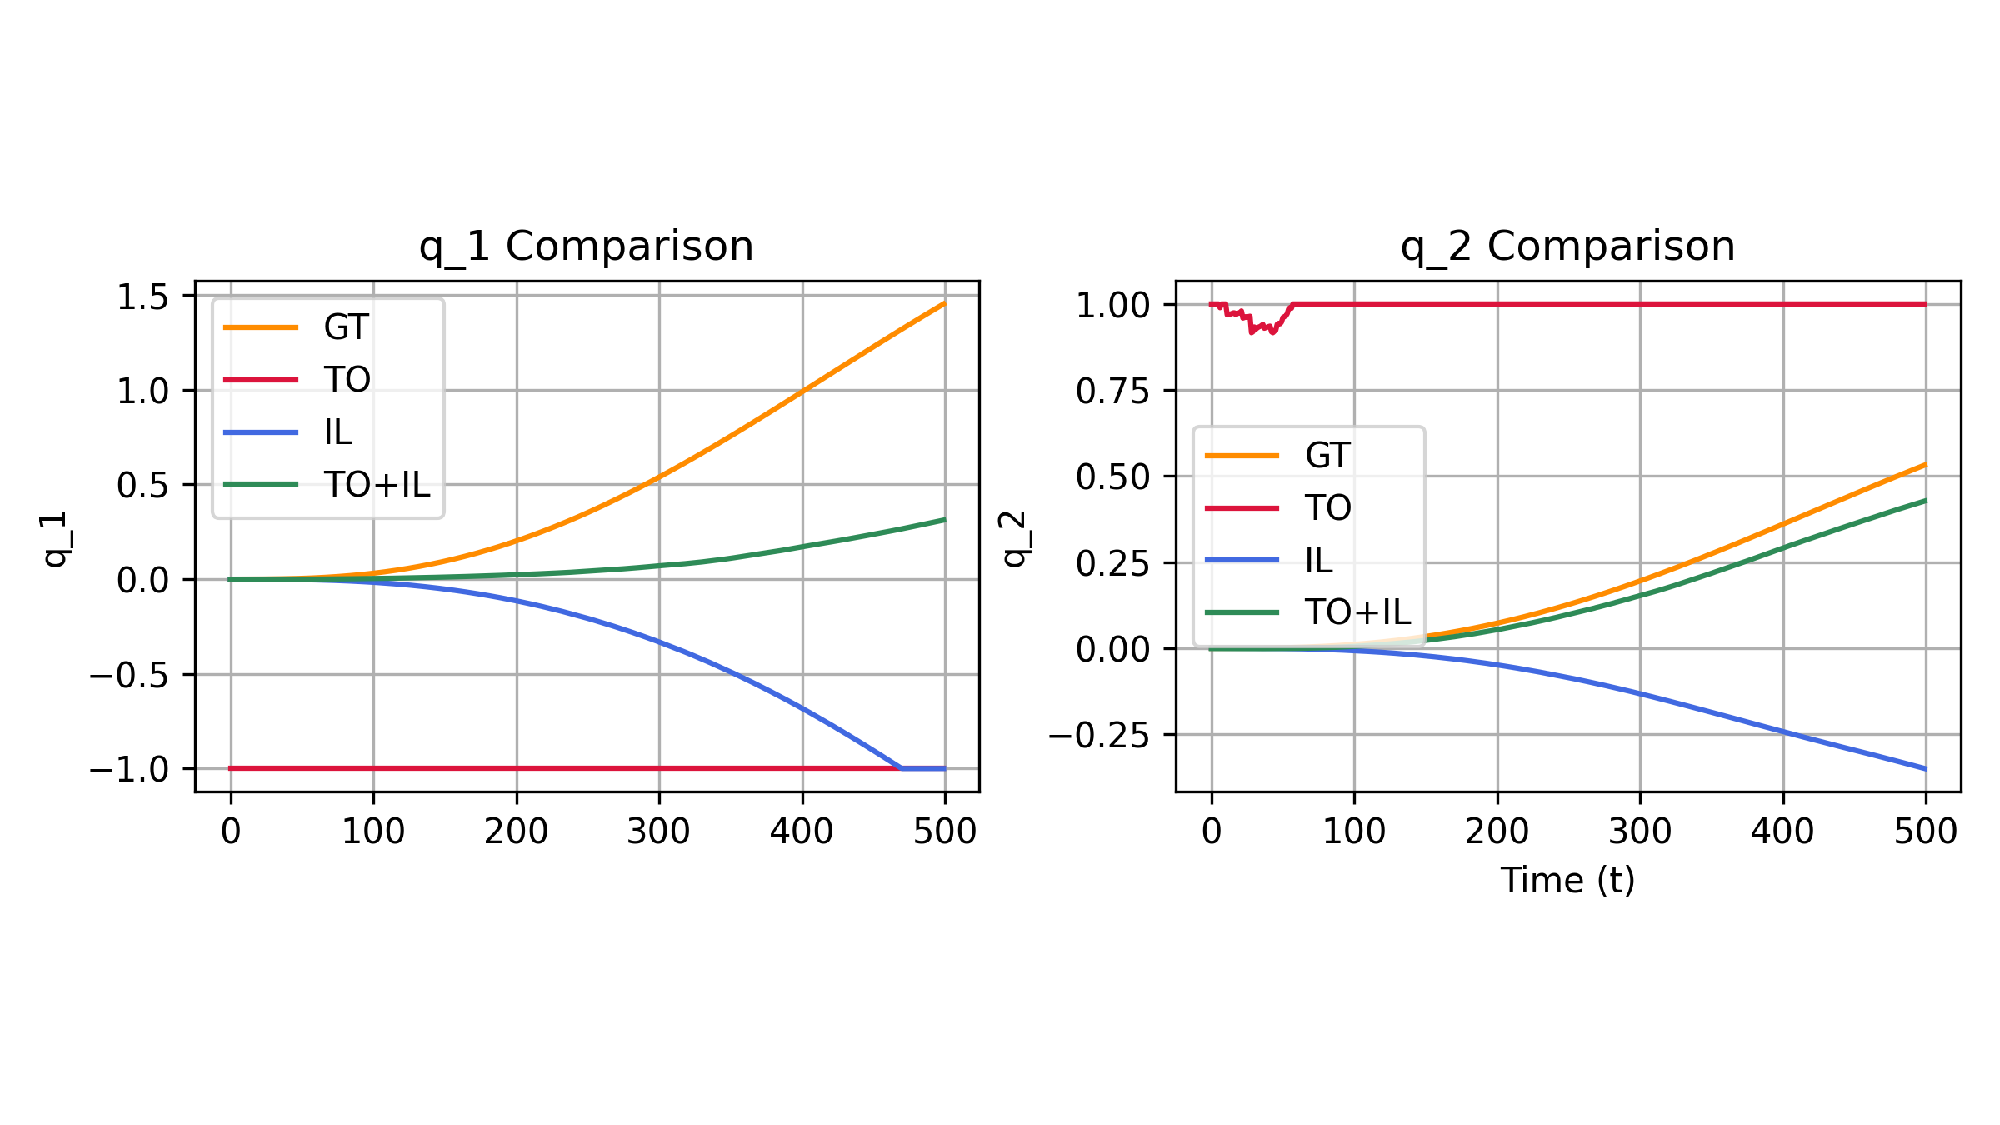
\includegraphics[width=0.95\linewidth]{./graph/IL_TO_comparison.pdf}
\captionof{figure}{A case study comparing learning strategies. TO improves IL's action accuracy but fails to produce correct actions on its own.}
\label{fig:IL_TO}
\end{minipage}
\vspace{-0.5cm}
\end{table}
 




\subsection{Ablation study on the Test-time Adaption.}


\begin{figure*}[t]
\centering
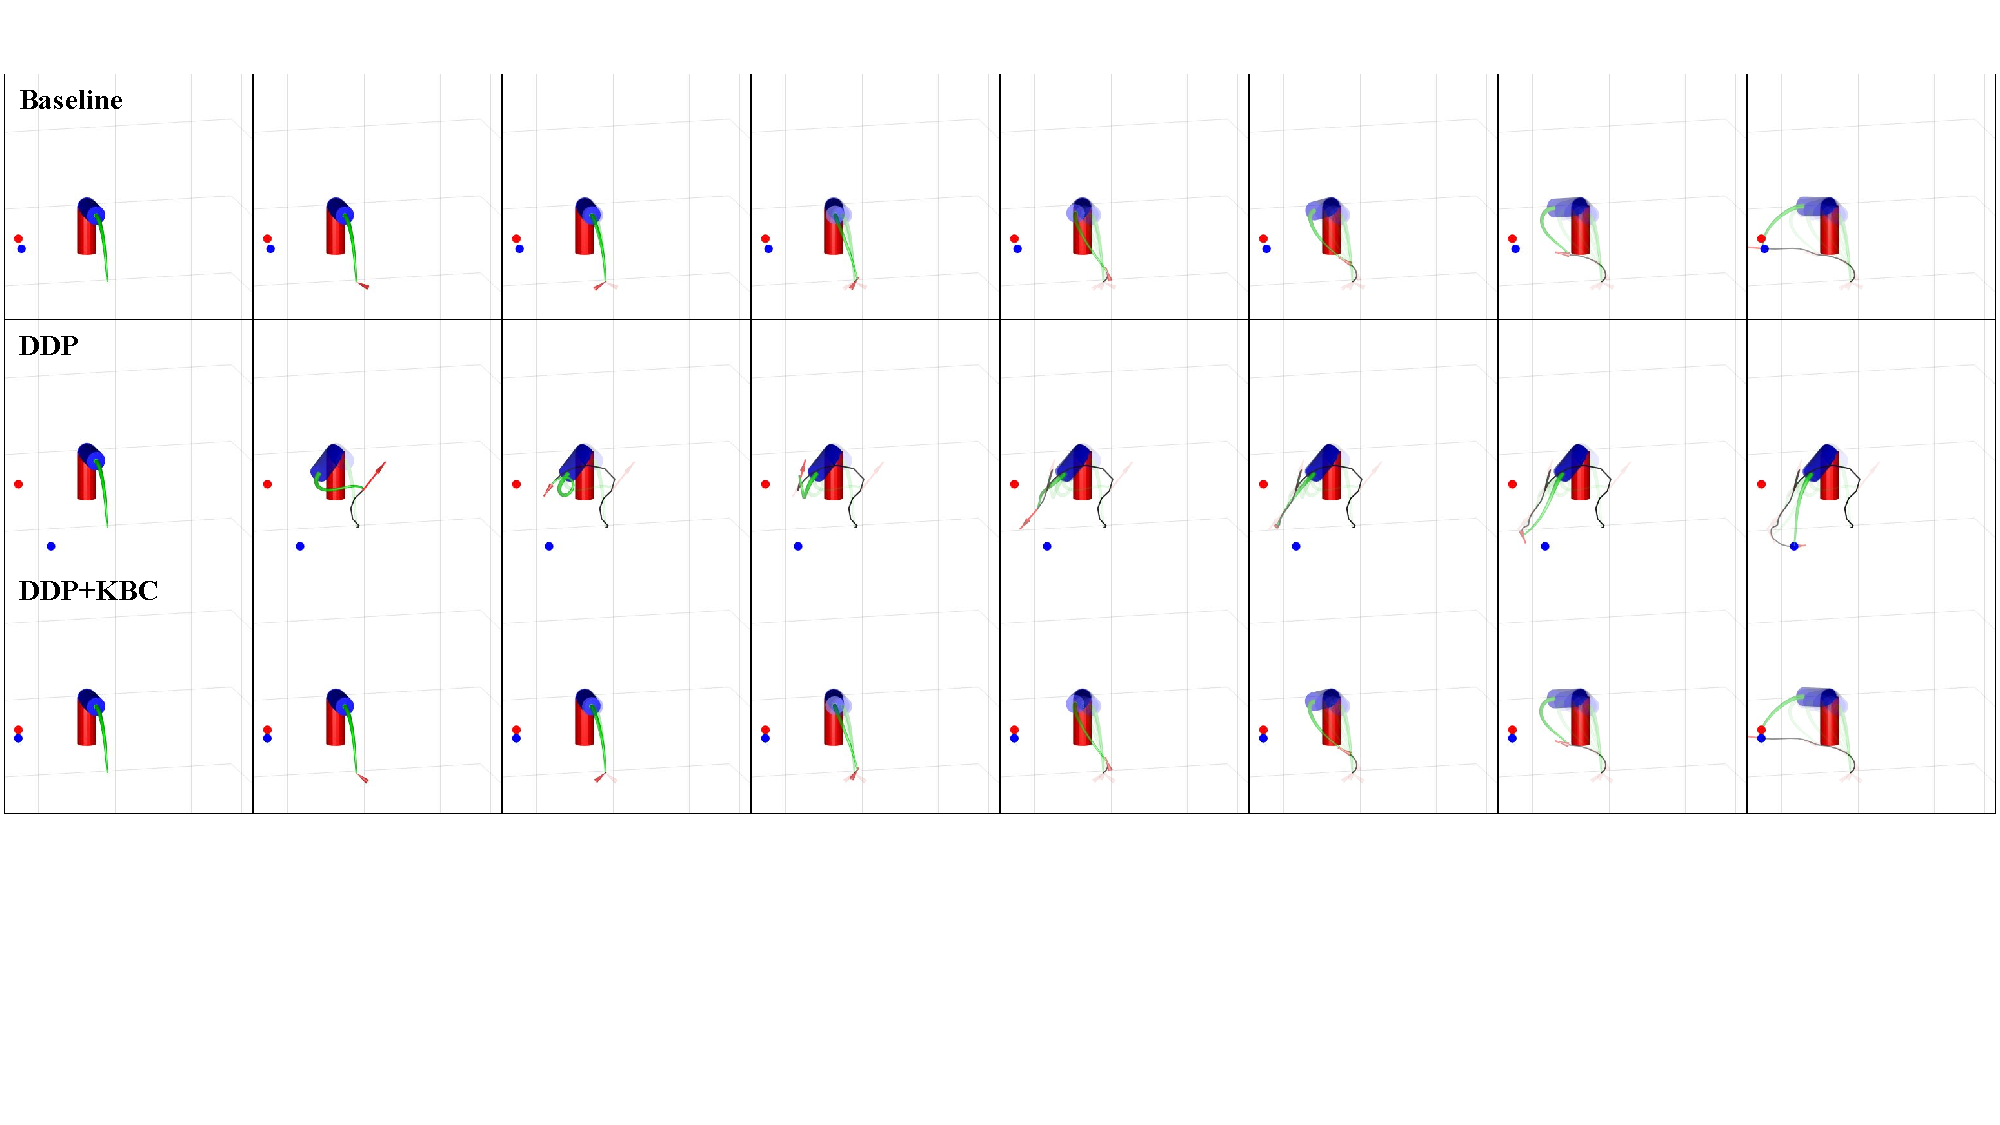
\includegraphics[width=0.95\linewidth]{./graph/tta_ada_ablation.pdf} 
\caption{Visualization of the manipulation process. The baseline represents the diffusion policy without test-time adaptation. \textbf{DDP} denotes test-time adaptation using only the differentiable dynamics prior, while \textbf{KBC} indicates adaptation incorporating the kinematic boundary condition.}
\vspace{-0.5cm}
\label{fig:tta_ablation}
\end{figure*}
\textbf{Experimental Settings.} We evaluate the effectiveness of the proposed test-time adaptation strategy by comparing different configurations:

\textit{Tuning Strategy.} We examine two approaches for updating model parameters during test-time adaptation. \textbf{Full Finetune} indicates that all parameters are fine-tuned during adaptation, while \textbf{Project Finetune} refers to freezing most of the model and updating only the final projection layer.

\textit{Physical Priors.} We assess the influence of incorporating physical constraints during test-time adaptation. \textit{DDP} denotes the use of a Differential Dynamics Prior to guide the adaptation process, and \textit{KBC} refers to enforcing Kinematic Boundary Conditions to ensure physically consistent outputs.


\textbf{Experimental Analysis.}
We observe that incorporating KBC is essential for maintaining consistency at the trajectory's initial state. As shown in Table~\ref{tab: phi_prior}, without KBC, test-time adaptation using DDP becomes unstable, often producing physically implausible motions and reduced task performance.
Moreover, different adaptation strategies during fine-tuning yield varied results. As shown in Table~\ref{tab: Tuning}, full finetuning incurs nearly 40\% additional inference time per sample while leading to a drop in overall performance. This degradation arises because updating the entire network often disrupts the behaviors learned during the imitation phase, negatively affecting both convergence and generalization. In contrast, restricting adaptation to the final projection layer offers a more favorable trade-off between flexibility and stability.


 


\begin{table}[ht]
\centering
\vspace{-0.4cm}
\begin{minipage}{0.49\textwidth}
\centering
\resizebox{\textwidth}{!}{
\begin{tabular}{cc|c|cccc}
\toprule
\multirow{2}{*}{DDP} & \multirow{2}{*}{KBC}             & \multirow{2}{*}{Distance} & \multicolumn{4}{c}{Success Rate}   \\ \cline{4-7}
    &   &             & 10 cm  & 5cm    & 2 cm   & 1 cm  \\ \midrule
      &                                     & 0.057                        & 0.884  & 0.800  & 0.616  & 0.190    \\ 
\checkmark &                     & 0.189                        & 0.304  & 0.124  & 0.038  & 0.020 \\
\checkmark &\checkmark     & 0.036                     & 0.939  & 0.843  & 0.623  & 0.208 \\ \midrule
\end{tabular} 
}
\caption{Ablation study on the choice of physical priors. KBC plays a crucial role in constraining the initial boundary states. When omitted during test-time adaptation with DDP, the policy suffers from unstable predictions, leading to a significantly lower success rate.}
\label{tab: phi_prior}

\end{minipage}
\hfill
\begin{minipage}{0.49\textwidth}
\centering
\resizebox{\textwidth}{!}{\begin{tabular}{c|c|c|cccc}
\toprule
\multirow{2}{*}{Tuning Strategy}  & \multirow{2}{*}{Time (s)}  & \multirow{2}{*}{Distance} & \multicolumn{4}{c}{Success Rate}   \\ \cline{4-7}
    &         &  & 10 cm  & 5 cm   & 2 cm   & 1 cm  \\ \midrule
Full Finetune  &  14.22  &  0.096     &  0.864 &0.678   &0.146   &0.020  \\
Project Finetune  & 10.39  & 0.036                     & 0.939  & 0.843  & 0.623  & 0.208 \\ \midrule
\end{tabular}}
\caption{Ablation study on the tuning strategy. Full finetuning tends to overwrite the knowledge learned during imitation pretraining, resulting in instability in the final policy. In contrast, projection-layer finetuning, which updates fewer parameters, preserves the pretrained behavior while enabling effective adaptation.}
\label{tab: Tuning}
\end{minipage}
\vspace{-0.5cm}
\end{table}

 
\subsection{Limitations.}
This work focuses primarily on learning the inverse dynamics of the entire system under a specific deformable object setup. However, it does not account for variations in object shape, material properties, or other physical characteristics that may significantly impact system behavior. As a result, the learned policy is tailored to a single type of deformable object, limiting its generalizability. In future work, we aim to address this limitation by expanding the dataset to include diverse deformable objects and incorporating object-specific attributes into the learning process. % Additionally, we plan to explore multi-task policy learning frameworks that can generalize across different object configurations, paving the way toward a more unified and robust manipulation strategy.

\section{Conclusion}

In this work, we present DIDP, a Dynamics-Informed Diffusion Policy framework for goal-conditioned dynamic manipulation of deformable objects in 3D environments. Our approach combines a reduced-order modeling formulation with a diffusion-based policy that incorporates physical priors through test-time adaptation. By modeling the inverse dynamics within a compact, task-relevant latent space, DIDP achieves efficient and physically grounded action generation. Extensive experiments demonstrate that DIDP outperforms existing baselines in terms of both accuracy and robustness. We believe this work offers a promising direction for bridging efficient learning and physically control in dynamic robotic manipulation.

%%%%%%%%%%%%%%%%%%%%%%%%%%%%%%%%%%%%%%%%%%%%%%%%%%%%%%%%%%%%

\setlength{\bibsep}{5pt}
%\bibliographystyle{plainnat}
%{\small \bibliography{main.bib}}
%{
{\small
\bibliographystyle{plain}
\bibliography{main}
}


\begin{comment}
%%%%%%%%%%%%%%%%%%%%%%%%%%%%%%%%%%%%%%%%%%%%%%%%%%%%%%%%%%%%
\newpage

\appendix

\section{Simulation Environments}%Matlab Code Link, Project Page Link 放着
This section outlines the simulation environments utilized for conducting the experiments. It provides an overview of the hardware configuration, software requirements, and any additional setup necessary for running the experiments.

\subsection{Software Requirements}
- MATLAB: R2023b or higher

- Additional Libraries:\href{https://github.com/SoRoSim/SoRoSim}{\textcolor{pretty-blue}{SoRoSim}}  

\subsection{Resources}
For further details, you can refer to the following resources:

Code Repository: \href{https://github.com/anonymousguy2025/DDIP}{\textcolor{pretty-blue}{[DDIP Code]}}  

Project Page: \href{https://anonymousguy2025.github.io/DDIP_project_page/}{\textcolor{pretty-blue}{[DDIP Project Page]}}  

\section{Implementation Details}

\subsection{Dataset Details}

The dataset comprises \textbf{55,000} high-fidelity simulated trajectories of a whip-like continuum soft robot. These trajectories are the result of simulating the robot's dynamics based on random actuation inputs, capturing the robot's motion across various configurations. Each trajectory is recorded over a duration of 2 seconds, with a fixed time step of 0.001 seconds, yielding 501 discrete time steps.

\textbf{HDF5 Structure:}
The dataset is organized into HDF5 files, with each file containing the following data fields. Each HDF5 file follows the naming convention \texttt{DynamicsSolution\_SoRoSim\_<k>.h5}, where \texttt{<k>} is the index of the dataset.

\begin{table}[ht]
\renewcommand{\arraystretch}{1.5} % 仅对这个表格生效，调整行间距
\centering
\begin{tabular}{|l|l|l|}
\hline
\textbf{Dataset }        & \textbf{Description}                                      & \textbf{Size} \\
\hline
\texttt{T}              & Time duration (Total duration 0.5s)                          & $1 \times 1$ \\
\hline
\texttt{all\_positions} & The positions of the robot/rope at each time step    & $501 \times 21$ \\
\hline
\texttt{all\_velocities}& The velocities of the robot/rope at each time step         & $501 \times 21$ \\
\hline
\texttt{qqd}            & Robot/Rope angles (\texttt{theta}) and angular velocities (\texttt{theta dot}) & $501 \times 40$ \\
\hline
\texttt{theta}          & The joint angles of the two actuated joints                   & $2 \times 4$ \\
\hline
\texttt{t}              & Time steps (Total duration 0.5s, divided into 501 steps)   & $501 \times 1$ \\
\hline
\end{tabular}
\caption{Dataset Details}
\label{tab:dataset_details}
\end{table}



\subsection{Testing}

To validate the system and verify its functionality, the following MATLAB driver script can be used:

\begin{verbatim}
Driver_NB_DIDP.
\end{verbatim}

This script will execute the simulation and ensure that all data fields, including time steps, joint velocities, angles, external forces/torques, as well as robot/rope positions and velocities, are correctly processed and integrated within the system.


\subsection{Network Design}
We adopt a Transformer-based architecture as the denoiser of the diffusion policy, incorporating both cross attention and causal attention to effectively model the temporal structure and goal-conditioning in action prediction tasks.

\textbf{Cross Attention for Conditioning. } To ensure the model generates goal-directed actions, we employ \textit{cross attention} layers that inject goal information into each denoising step. 

\textbf{Autoregressive Action Prediction. } 
From a sequential modeling perspective, the generation process naturally follows an \textit{autoregressive factorization} of the conditional distribution:
\begin{equation}
    p(\bm{Q}_t \mid \bm{P}) = \prod_{i=1}^{T} p(\boldsymbol{q}_i \mid \boldsymbol{q}_{<i}, \bm{P})
\end{equation}

To capture this structure within our Transformer-based denoiser, we employ \textbf{causal self-attention}, which ensures that each token $\boldsymbol{q}_i$ attends only to itself and preceding tokens $\{\boldsymbol{q}_1, \dots, \boldsymbol{q}_{i-1}\}$. This structure is particularly suitable for modeling sequences of actions, where temporal causality must be strictly preserved for realistic and physically valid generation.
\subsection{Training Details}
We train our policy for 2 million iterations with the framwork of Transformer-based diffusion model on the Gaussian flow.  We employ the Adam optimizer with a learning rate of $1 \times 10^{-4}$, applying linear weight decay. To stabilize training, we utilize an exponential moving average (EMA) with a weight of 0.9999 during parameter updates in both the pretrain and distillation stages. We adopt a fine-grained diffusion method with $T = 512$ steps and implement a linear noise schedule with endpoints set at $1 \times 10^{-4}$ and $2 \times 10^{-2}$. All the experiments are run on a single 3090 GPU with 24GB of memory. Training our method with a smaller patch size and batch size on a device with less memory is feasible.



 



\begin{figure*}[t]
\centering
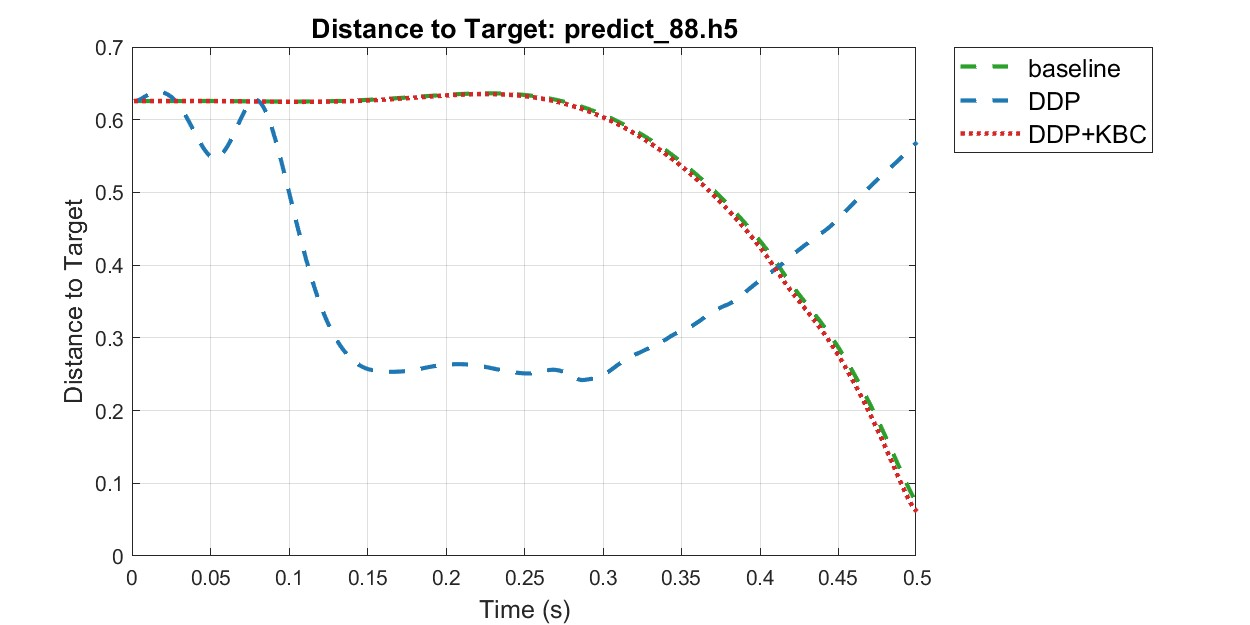
\includegraphics[width=0.95\linewidth]{./graph/predict_88.jpg} 
\caption{This plot illustrates the distance to the target over time for three different approaches: baseline, DDP (Differential Dynamic Prior), and DDP+KBC (DDP with Kinematic Boundary Conditions). The x-axis represents time (in seconds), and the y-axis shows the distance to target.}
\vspace{-0.5cm}
\label{fig:tta_ablation_curve}
\end{figure*}


    

\newpage
\section*{NeurIPS Paper Checklist}

%%% BEGIN INSTRUCTIONS %%%
The checklist is designed to encourage best practices for responsible machine learning research, addressing issues of reproducibility, transparency, research ethics, and societal impact. Do not remove the checklist: {\bf The papers not including the checklist will be desk rejected.} The checklist should follow the references and follow the (optional) supplemental material.  The checklist does NOT count towards the page
limit. 

Please read the checklist guidelines carefully for information on how to answer these questions. For each question in the checklist:
\begin{itemize}
    \item You should answer \answerYes{}, \answerNo{}, or \answerNA{}.
    \item \answerNA{} means either that the question is Not Applicable for that particular paper or the relevant information is Not Available.
    \item Please provide a short (1–2 sentence) justification right after your answer (even for NA). 
   % \item {\bf The papers not including the checklist will be desk rejected.}
\end{itemize}

{\bf The checklist answers are an integral part of your paper submission.} They are visible to the reviewers, area chairs, senior area chairs, and ethics reviewers. You will be asked to also include it (after eventual revisions) with the final version of your paper, and its final version will be published with the paper.

The reviewers of your paper will be asked to use the checklist as one of the factors in their evaluation. While "\answerYes{}" is generally preferable to "\answerNo{}", it is perfectly acceptable to answer "\answerNo{}" provided a proper justification is given (e.g., "error bars are not reported because it would be too computationally expensive" or "we were unable to find the license for the dataset we used"). In general, answering "\answerNo{}" or "\answerNA{}" is not grounds for rejection. While the questions are phrased in a binary way, we acknowledge that the true answer is often more nuanced, so please just use your best judgment and write a justification to elaborate. All supporting evidence can appear either in the main paper or the supplemental material, provided in appendix. If you answer \answerYes{} to a question, in the justification please point to the section(s) where related material for the question can be found.

IMPORTANT, please:
\begin{itemize}
    \item {\bf Delete this instruction block, but keep the section heading ``NeurIPS Paper Checklist"},
    \item  {\bf Keep the checklist subsection headings, questions/answers and guidelines below.}
    \item {\bf Do not modify the questions and only use the provided macros for your answers}.
\end{itemize} 
 

%%% END INSTRUCTIONS %%%


\begin{enumerate}

\item {\bf Claims}
    \item[] Question: Do the main claims made in the abstract and introduction accurately reflect the paper's contributions and scope?
    \item[] Answer: \answerYes{} % Replace by \answerYes{}, \answerNo{}, or \answerNA{}.
    \item[] Justification: The abstract and introduction should clearly state the contributions made in the paper.
    \item[] Guidelines:
    \begin{itemize}
        \item The answer NA means that the abstract and introduction do not include the claims made in the paper.
        \item The abstract and/or introduction should clearly state the claims made, including the contributions made in the paper and important assumptions and limitations. A No or NA answer to this question will not be perceived well by the reviewers. 
        \item The claims made should match theoretical and experimental results, and reflect how much the results can be expected to generalize to other settings. 
        \item It is fine to include aspirational goals as motivation as long as it is clear that these goals are not attained by the paper. 
    \end{itemize}

\item {\bf Limitations}
    \item[] Question: Does the paper discuss the limitations of the work performed by the authors?
    \item[] Answer: \answerYes{}% Replace by \answerYes{}, \answerNo{}, or \answerNA{}.
    \item[] Justification: Please refer to the "Limitations" section.
    \item[] Guidelines:
    \begin{itemize}
        \item The answer NA means that the paper has no limitation while the answer No means that the paper has limitations, but those are not discussed in the paper. 
        \item The authors are encouraged to create a separate "Limitations" section in their paper.
        \item The paper should point out any strong assumptions and how robust the results are to violations of these assumptions (e.g., independence assumptions, noiseless settings, model well-specification, asymptotic approximations only holding locally). The authors should reflect on how these assumptions might be violated in practice and what the implications would be.
        \item The authors should reflect on the scope of the claims made, e.g., if the approach was only tested on a few datasets or with a few runs. In general, empirical results often depend on implicit assumptions, which should be articulated.
        \item The authors should reflect on the factors that influence the performance of the approach. For example, a facial recognition algorithm may perform poorly when image resolution is low or images are taken in low lighting. Or a speech-to-text system might not be used reliably to provide closed captions for online lectures because it fails to handle technical jargon.
        \item The authors should discuss the computational efficiency of the proposed algorithms and how they scale with dataset size.
        \item If applicable, the authors should discuss possible limitations of their approach to address problems of privacy and fairness.
        \item While the authors might fear that complete honesty about limitations might be used by reviewers as grounds for rejection, a worse outcome might be that reviewers discover limitations that aren't acknowledged in the paper. The authors should use their best judgment and recognize that individual actions in favor of transparency play an important role in developing norms that preserve the integrity of the community. Reviewers will be specifically instructed to not penalize honesty concerning limitations.
    \end{itemize}

\item {\bf Theory assumptions and proofs}
    \item[] Question: For each theoretical result, does the paper provide the full set of assumptions and a complete (and correct) proof?
    \item[] Answer: \answerYes{} % Replace by \answerYes{}, \answerNo{}, or \answerNA{}.
    \item[] Justification: The paper provide the full set of assumptions and a complete (and correct) proof
    \item[] Guidelines:
    \begin{itemize}
        \item The answer NA means that the paper does not include theoretical results. 
        \item All the theorems, formulas, and proofs in the paper should be numbered and cross-referenced.
        \item All assumptions should be clearly stated or referenced in the statement of any theorems.
        \item The proofs can either appear in the main paper or the supplemental material, but if they appear in the supplemental material, the authors are encouraged to provide a short proof sketch to provide intuition. 
        \item Inversely, any informal proof provided in the core of the paper should be complemented by formal proofs provided in appendix or supplemental material.
        \item Theorems and Lemmas that the proof relies upon should be properly referenced. 
    \end{itemize}

    \item {\bf Experimental result reproducibility}
    \item[] Question: Does the paper fully disclose all the information needed to reproduce the main experimental results of the paper to the extent that it affects the main claims and/or conclusions of the paper (regardless of whether the code and data are provided or not)?
    \item[] Answer: \answerYes{}  % Replace by \answerYes{}, \answerNo{}, or \answerNA{}.
    \item[] Justification: The implementation details are provided in the supplementary material.
    \item[] Guidelines:
    \begin{itemize}
        \item The answer NA means that the paper does not include experiments.
        \item If the paper includes experiments, a No answer to this question will not be perceived well by the reviewers: Making the paper reproducible is important, regardless of whether the code and data are provided or not.
        \item If the contribution is a dataset and/or model, the authors should describe the steps taken to make their results reproducible or verifiable. 
        \item Depending on the contribution, reproducibility can be accomplished in various ways. For example, if the contribution is a novel architecture, describing the architecture fully might suffice, or if the contribution is a specific model and empirical evaluation, it may be necessary to either make it possible for others to replicate the model with the same dataset, or provide access to the model. In general. releasing code and data is often one good way to accomplish this, but reproducibility can also be provided via detailed instructions for how to replicate the results, access to a hosted model (e.g., in the case of a large language model), releasing of a model checkpoint, or other means that are appropriate to the research performed.
        \item While NeurIPS does not require releasing code, the conference does require all submissions to provide some reasonable avenue for reproducibility, which may depend on the nature of the contribution. For example
        \begin{enumerate}
            \item If the contribution is primarily a new algorithm, the paper should make it clear how to reproduce that algorithm.
            \item If the contribution is primarily a new model architecture, the paper should describe the architecture clearly and fully.
            \item If the contribution is a new model (e.g., a large language model), then there should either be a way to access this model for reproducing the results or a way to reproduce the model (e.g., with an open-source dataset or instructions for how to construct the dataset).
            \item We recognize that reproducibility may be tricky in some cases, in which case authors are welcome to describe the particular way they provide for reproducibility. In the case of closed-source models, it may be that access to the model is limited in some way (e.g., to registered users), but it should be possible for other researchers to have some path to reproducing or verifying the results.
        \end{enumerate}
    \end{itemize}


\item {\bf Open access to data and code}
    \item[] Question: Does the paper provide open access to the data and code, with sufficient instructions to faithfully reproduce the main experimental results, as described in supplemental material?
    \item[] Answer: \answerYes{} % Replace by \answerYes{}, \answerNo{}, or \answerNA{}.
    \item[] Justification: We provide the code link.
    \item[] Guidelines:
    \begin{itemize}
        \item The answer NA means that paper does not include experiments requiring code.
        \item Please see the NeurIPS code and data submission guidelines (\url{https://nips.cc/public/guides/CodeSubmissionPolicy}) for more details.
        \item While we encourage the release of code and data, we understand that this might not be possible, so “No” is an acceptable answer. Papers cannot be rejected simply for not including code, unless this is central to the contribution (e.g., for a new open-source benchmark).
        \item The instructions should contain the exact command and environment needed to run to reproduce the results. See the NeurIPS code and data submission guidelines (\url{https://nips.cc/public/guides/CodeSubmissionPolicy}) for more details.
        \item The authors should provide instructions on data access and preparation, including how to access the raw data, preprocessed data, intermediate data, and generated data, etc.
        \item The authors should provide scripts to reproduce all experimental results for the new proposed method and baselines. If only a subset of experiments are reproducible, they should state which ones are omitted from the script and why.
        \item At submission time, to preserve anonymity, the authors should release anonymized versions (if applicable).
        \item Providing as much information as possible in supplemental material (appended to the paper) is recommended, but including URLs to data and code is permitted.
    \end{itemize}


\item {\bf Experimental setting/details}
    \item[] Question: Does the paper specify all the training and test details (e.g., data splits, hyperparameters, how they were chosen, type of optimizer, etc.) necessary to understand the results?
    \item[] Answer: \answerYes{} % Replace by \answerYes{}, \answerNo{}, or \answerNA{}.
    \item[] Justification: The implementation details are provided in the supplementary material.
    \item[] Guidelines: 
    \begin{itemize}
        \item The answer NA means that the paper does not include experiments.
        \item The experimental setting should be presented in the core of the paper to a level of detail that is necessary to appreciate the results and make sense of them.
        \item The full details can be provided either with the code, in appendix, or as supplemental material.
    \end{itemize}

\item {\bf Experiment statistical significance}
    \item[] Question: Does the paper report error bars suitably and correctly defined or other appropriate information about the statistical significance of the experiments?
    \item[] Answer:  \answerNo{} % Replace by \answerYes{}, \answerNo{}, or \answerNA{}.
    \item[] Justification: Results without error bars.
    \item[] Guidelines:
    \begin{itemize}
        \item The answer NA means that the paper does not include experiments.
        \item The authors should answer "Yes" if the results are accompanied by error bars, confidence intervals, or statistical significance tests, at least for the experiments that support the main claims of the paper.
        \item The factors of variability that the error bars are capturing should be clearly stated (for example, train/test split, initialization, random drawing of some parameter, or overall run with given experimental conditions).
        \item The method for calculating the error bars should be explained (closed form formula, call to a library function, bootstrap, etc.)
        \item The assumptions made should be given (e.g., Normally distributed errors).
        \item It should be clear whether the error bar is the standard deviation or the standard error of the mean.
        \item It is OK to report 1-sigma error bars, but one should state it. The authors should preferably report a 2-sigma error bar than state that they have a 96\% CI, if the hypothesis of Normality of errors is not verified.
        \item For asymmetric distributions, the authors should be careful not to show in tables or figures symmetric error bars that would yield results that are out of range (e.g. negative error rates).
        \item If error bars are reported in tables or plots, The authors should explain in the text how they were calculated and reference the corresponding figures or tables in the text.
    \end{itemize}

\item {\bf Experiments compute resources}
    \item[] Question: For each experiment, does the paper provide sufficient information on the computer resources (type of compute workers, memory, time of execution) needed to reproduce the experiments?
    \item[] Answer:\answerYes{} % Replace by \answerYes{}, \answerNo{}, or \answerNA{}.
    \item[] Justification: Refer to the Supp.
    \item[] Guidelines:
    \begin{itemize}
        \item The answer NA means that the paper does not include experiments.
        \item The paper should indicate the type of compute workers CPU or GPU, internal cluster, or cloud provider, including relevant memory and storage.
        \item The paper should provide the amount of compute required for each of the individual experimental runs as well as estimate the total compute. 
        \item The paper should disclose whether the full research project required more compute than the experiments reported in the paper (e.g., preliminary or failed experiments that didn't make it into the paper). 
    \end{itemize}
    
\item {\bf Code of ethics}
    \item[] Question: Does the research conducted in the paper conform, in every respect, with the NeurIPS Code of Ethics \url{https://neurips.cc/public/EthicsGuidelines}?
    \item[] Answer: \answerYes{}  % Replace by \answerYes{}, \answerNo{}, or \answerNA{}.
    \item[] Justification: Yes.
    \item[] Guidelines:
    \begin{itemize}
        \item The answer NA means that the authors have not reviewed the NeurIPS Code of Ethics.
        \item If the authors answer No, they should explain the special circumstances that require a deviation from the Code of Ethics.
        \item The authors should make sure to preserve anonymity (e.g., if there is a special consideration due to laws or regulations in their jurisdiction).
    \end{itemize}


\item {\bf Broader impacts}
    \item[] Question: Does the paper discuss both potential positive societal impacts and negative societal impacts of the work performed?
    \item[] Answer: \answerYes{} % Replace by \answerYes{}, \answerNo{}, or \answerNA{}.
    \item[] Justification: Refer to the introduction and conclusion.
    \item[] Guidelines:
    \begin{itemize}
        \item The answer NA means that there is no societal impact of the work performed.
        \item If the authors answer NA or No, they should explain why their work has no societal impact or why the paper does not address societal impact.
        \item Examples of negative societal impacts include potential malicious or unintended uses (e.g., disinformation, generating fake profiles, surveillance), fairness considerations (e.g., deployment of technologies that could make decisions that unfairly impact specific groups), privacy considerations, and security considerations.
        \item The conference expects that many papers will be foundational research and not tied to particular applications, let alone deployments. However, if there is a direct path to any negative applications, the authors should point it out. For example, it is legitimate to point out that an improvement in the quality of generative models could be used to generate deepfakes for disinformation. On the other hand, it is not needed to point out that a generic algorithm for optimizing neural networks could enable people to train models that generate Deepfakes faster.
        \item The authors should consider possible harms that could arise when the technology is being used as intended and functioning correctly, harms that could arise when the technology is being used as intended but gives incorrect results, and harms following from (intentional or unintentional) misuse of the technology.
        \item If there are negative societal impacts, the authors could also discuss possible mitigation strategies (e.g., gated release of models, providing defenses in addition to attacks, mechanisms for monitoring misuse, mechanisms to monitor how a system learns from feedback over time, improving the efficiency and accessibility of ML).
    \end{itemize}
    
\item {\bf Safeguards}
    \item[] Question: Does the paper describe safeguards that have been put in place for responsible release of data or models that have a high risk for misuse (e.g., pretrained language models, image generators, or scraped datasets)?
    \item[] Answer:\answerYes{} % Replace by \answerYes{}, \answerNo{}, or \answerNA{}.
    \item[] Justification: Refer to the Supp.
    \item[] Guidelines:
    \begin{itemize}
        \item The answer NA means that the paper poses no such risks.
        \item Released models that have a high risk for misuse or dual-use should be released with necessary safeguards to allow for controlled use of the model, for example by requiring that users adhere to usage guidelines or restrictions to access the model or implementing safety filters. 
        \item Datasets that have been scraped from the Internet could pose safety risks. The authors should describe how they avoided releasing unsafe images.
        \item We recognize that providing effective safeguards is challenging, and many papers do not require this, but we encourage authors to take this into account and make a best faith effort.
    \end{itemize}

\item {\bf Licenses for existing assets}
    \item[] Question: Are the creators or original owners of assets (e.g., code, data, models), used in the paper, properly credited and are the license and terms of use explicitly mentioned and properly respected?
    \item[] Answer: \answerYes{} % Replace by \answerYes{}, \answerNo{}, or \answerNA{}.
    \item[] Justification: Al the related works are properly credited.
    \item[] Guidelines:
    \begin{itemize}
        \item The answer NA means that the paper does not use existing assets.
        \item The authors should cite the original paper that produced the code package or dataset.
        \item The authors should state which version of the asset is used and, if possible, include a URL.
        \item The name of the license (e.g., CC-BY 4.0) should be included for each asset.
        \item For scraped data from a particular source (e.g., website), the copyright and terms of service of that source should be provided.
        \item If assets are released, the license, copyright information, and terms of use in the package should be provided. For popular datasets, \url{paperswithcode.com/datasets} has curated licenses for some datasets. Their licensing guide can help determine the license of a dataset.
        \item For existing datasets that are re-packaged, both the original license and the license of the derived asset (if it has changed) should be provided.
        \item If this information is not available online, the authors are encouraged to reach out to the asset's creators.
    \end{itemize}

\item {\bf New assets}
    \item[] Question: Are new assets introduced in the paper well documented and is the documentation provided alongside the assets?
    \item[] Answer:  \answerYes{}  % Replace by \answerYes{}, \answerNo{}, or \answerNA{}.
    \item[] Justification:  New assets introduced in the paper are well documented.
    \item[] Guidelines:
    \begin{itemize}
        \item The answer NA means that the paper does not release new assets.
        \item Researchers should communicate the details of the dataset/code/model as part of their submissions via structured templates. This includes details about training, license, limitations, etc. 
        \item The paper should discuss whether and how consent was obtained from people whose asset is used.
        \item At submission time, remember to anonymize your assets (if applicable). You can either create an anonymized URL or include an anonymized zip file.
    \end{itemize}

\item {\bf Crowdsourcing and research with human subjects}
    \item[] Question: For crowdsourcing experiments and research with human subjects, does the paper include the full text of instructions given to participants and screenshots, if applicable, as well as details about compensation (if any)? 
    \item[] Answer: \answerNA{} % Replace by \answerYes{}, \answerNo{}, or \answerNA{}.
    \item[] Justification: The paper does not involve crowdsourcing nor research with human subjects.
    \item[] Guidelines:
    \begin{itemize}
        \item The answer NA means that the paper does not involve crowdsourcing nor research with human subjects.
        \item Including this information in the supplemental material is fine, but if the main contribution of the paper involves human subjects, then as much detail as possible should be included in the main paper. 
        \item According to the NeurIPS Code of Ethics, workers involved in data collection, curation, or other labor should be paid at least the minimum wage in the country of the data collector. 
    \end{itemize}

\item {\bf Institutional review board (IRB) approvals or equivalent for research with human subjects}
    \item[] Question: Does the paper describe potential risks incurred by study participants, whether such risks were disclosed to the subjects, and whether Institutional Review Board (IRB) approvals (or an equivalent approval/review based on the requirements of your country or institution) were obtained?
    \item[] Answer: \answerNA{} % Replace by \answerYes{}, \answerNo{}, or \answerNA{}.
    \item[] Justification: The paper does not involve crowdsourcing nor research with human subjects.
    \item[] Guidelines:
    \begin{itemize}
        \item The answer NA means that the paper does not involve crowdsourcing nor research with human subjects.
        \item Depending on the country in which research is conducted, IRB approval (or equivalent) may be required for any human subjects research. If you obtained IRB approval, you should clearly state this in the paper. 
        \item We recognize that the procedures for this may vary significantly between institutions and locations, and we expect authors to adhere to the NeurIPS Code of Ethics and the guidelines for their institution. 
        \item For initial submissions, do not include any information that would break anonymity (if applicable), such as the institution conducting the review.
    \end{itemize}

\item {\bf Declaration of LLM usage}
    \item[] Question: Does the paper describe the usage of LLMs if it is an important, original, or non-standard component of the core methods in this research? Note that if the LLM is used only for writing, editing, or formatting purposes and does not impact the core methodology, scientific rigorousness, or originality of the research, declaration is not required.
    %this research? 
    \item[] Answer: \answerYes{} % Replace by \answerYes{}, \answerNo{}, or \answerNA{}.
    \item[] Justification: LLM is used only for writing and editing.
    \item[] Guidelines:
    \begin{itemize}
        \item The answer NA means that the core method development in this research does not involve LLMs as any important, original, or non-standard components.
        \item Please refer to our LLM policy (\url{https://neurips.cc/Conferences/2025/LLM}) for what should or should not be described.
    \end{itemize}

\end{enumerate}

\end{comment}
\end{document}